% Options for packages loaded elsewhere
\PassOptionsToPackage{unicode}{hyperref}
\PassOptionsToPackage{hyphens}{url}
\PassOptionsToPackage{dvipsnames,svgnames,x11names}{xcolor}
%
\documentclass[
  authoryear,
  preprint,
  3p,
  onecolumn]{elsarticle}

\usepackage{amsmath,amssymb}
\usepackage{iftex}
\ifPDFTeX
  \usepackage[T1]{fontenc}
  \usepackage[utf8]{inputenc}
  \usepackage{textcomp} % provide euro and other symbols
\else % if luatex or xetex
  \usepackage{unicode-math}
  \defaultfontfeatures{Scale=MatchLowercase}
  \defaultfontfeatures[\rmfamily]{Ligatures=TeX,Scale=1}
\fi
\usepackage{lmodern}
\ifPDFTeX\else  
    % xetex/luatex font selection
\fi
% Use upquote if available, for straight quotes in verbatim environments
\IfFileExists{upquote.sty}{\usepackage{upquote}}{}
\IfFileExists{microtype.sty}{% use microtype if available
  \usepackage[]{microtype}
  \UseMicrotypeSet[protrusion]{basicmath} % disable protrusion for tt fonts
}{}
\makeatletter
\@ifundefined{KOMAClassName}{% if non-KOMA class
  \IfFileExists{parskip.sty}{%
    \usepackage{parskip}
  }{% else
    \setlength{\parindent}{0pt}
    \setlength{\parskip}{6pt plus 2pt minus 1pt}}
}{% if KOMA class
  \KOMAoptions{parskip=half}}
\makeatother
\usepackage{xcolor}
\setlength{\emergencystretch}{3em} % prevent overfull lines
\setcounter{secnumdepth}{5}
% Make \paragraph and \subparagraph free-standing
\ifx\paragraph\undefined\else
  \let\oldparagraph\paragraph
  \renewcommand{\paragraph}[1]{\oldparagraph{#1}\mbox{}}
\fi
\ifx\subparagraph\undefined\else
  \let\oldsubparagraph\subparagraph
  \renewcommand{\subparagraph}[1]{\oldsubparagraph{#1}\mbox{}}
\fi


\providecommand{\tightlist}{%
  \setlength{\itemsep}{0pt}\setlength{\parskip}{0pt}}\usepackage{longtable,booktabs,array}
\usepackage{calc} % for calculating minipage widths
% Correct order of tables after \paragraph or \subparagraph
\usepackage{etoolbox}
\makeatletter
\patchcmd\longtable{\par}{\if@noskipsec\mbox{}\fi\par}{}{}
\makeatother
% Allow footnotes in longtable head/foot
\IfFileExists{footnotehyper.sty}{\usepackage{footnotehyper}}{\usepackage{footnote}}
\makesavenoteenv{longtable}
\usepackage{graphicx}
\makeatletter
\def\maxwidth{\ifdim\Gin@nat@width>\linewidth\linewidth\else\Gin@nat@width\fi}
\def\maxheight{\ifdim\Gin@nat@height>\textheight\textheight\else\Gin@nat@height\fi}
\makeatother
% Scale images if necessary, so that they will not overflow the page
% margins by default, and it is still possible to overwrite the defaults
% using explicit options in \includegraphics[width, height, ...]{}
\setkeys{Gin}{width=\maxwidth,height=\maxheight,keepaspectratio}
% Set default figure placement to htbp
\makeatletter
\def\fps@figure{htbp}
\makeatother

\usepackage{lineno}\linenumbers \usepackage{multirow} \usepackage{lscape} \newcommand{\blandscape}{\begin{landscape}} \newcommand{\elandscape}{\end{landscape}}
\makeatletter
\makeatother
\makeatletter
\makeatother
\makeatletter
\@ifpackageloaded{caption}{}{\usepackage{caption}}
\AtBeginDocument{%
\ifdefined\contentsname
  \renewcommand*\contentsname{Table of contents}
\else
  \newcommand\contentsname{Table of contents}
\fi
\ifdefined\listfigurename
  \renewcommand*\listfigurename{List of Figures}
\else
  \newcommand\listfigurename{List of Figures}
\fi
\ifdefined\listtablename
  \renewcommand*\listtablename{List of Tables}
\else
  \newcommand\listtablename{List of Tables}
\fi
\ifdefined\figurename
  \renewcommand*\figurename{Figure}
\else
  \newcommand\figurename{Figure}
\fi
\ifdefined\tablename
  \renewcommand*\tablename{Table}
\else
  \newcommand\tablename{Table}
\fi
}
\@ifpackageloaded{float}{}{\usepackage{float}}
\floatstyle{ruled}
\@ifundefined{c@chapter}{\newfloat{codelisting}{h}{lop}}{\newfloat{codelisting}{h}{lop}[chapter]}
\floatname{codelisting}{Listing}
\newcommand*\listoflistings{\listof{codelisting}{List of Listings}}
\makeatother
\makeatletter
\@ifpackageloaded{caption}{}{\usepackage{caption}}
\@ifpackageloaded{subcaption}{}{\usepackage{subcaption}}
\makeatother
\makeatletter
\@ifpackageloaded{tcolorbox}{}{\usepackage[skins,breakable]{tcolorbox}}
\makeatother
\makeatletter
\@ifundefined{shadecolor}{\definecolor{shadecolor}{rgb}{.97, .97, .97}}
\makeatother
\makeatletter
\makeatother
\makeatletter
\makeatother
\journal{Journal Name}
\ifLuaTeX
  \usepackage{selnolig}  % disable illegal ligatures
\fi
\usepackage[]{natbib}
\bibliographystyle{elsarticle-harv}
\IfFileExists{bookmark.sty}{\usepackage{bookmark}}{\usepackage{hyperref}}
\IfFileExists{xurl.sty}{\usepackage{xurl}}{} % add URL line breaks if available
\urlstyle{same} % disable monospaced font for URLs
\hypersetup{
  pdftitle={The effects of multi-dimensional drought on land cover change and vegetation productivity in continental Chile},
  pdfauthor={Francisco Zambrano; Anton Vrieling; Francisco Meza; Iongel Duran-Llacer; Francisco Fernández; Alejandro Venegas-González; Nicolas Raab; Dylan Craven},
  pdfkeywords={drought, land cover change, satellite},
  colorlinks=true,
  linkcolor={blue},
  filecolor={Maroon},
  citecolor={Blue},
  urlcolor={Blue},
  pdfcreator={LaTeX via pandoc}}

\setlength{\parindent}{6pt}
\begin{document}

\begin{frontmatter}
\title{The effects of multi-dimensional drought on land cover change and
vegetation productivity in continental Chile}
\author[1]{Francisco Zambrano%
\corref{cor1}%
\fnref{fn1}}
 \ead{francisco.zambrano@umayor.cl} 
\author[2]{Anton Vrieling%
%
}
 \ead{a.vrieling@utwente.nl} 
\author[]{Francisco Meza%
%
}

\author[]{Iongel Duran-Llacer%
%
}

\author[3]{Francisco Fernández%
%
}
 \ead{francisco.fernandez@uss.cl} 
\author[]{Alejandro Venegas-González%
%
}

\author[]{Nicolas Raab%
%
}

\author[]{Dylan Craven%
%
}


\affiliation[1]{organization={Universidad Mayor, Hémera Centro de
Observación de la Tierra, Facultad de Ciencias, Escuela de Ingeniería en
Medio Ambiente y Sustentabilidad},city={Santiago,
Chile},postcode={7500994},postcodesep={}}
\affiliation[2]{organization={University of Twente, Faculty of
Geo-Information Science and Earth Observation (ITC)},city={Enschede, The
Netherlands},postcodesep={}}
\affiliation[3]{organization={Universidad San
Sebastian},,postcodesep={}}

\cortext[cor1]{Corresponding author}
\fntext[fn1]{This is the first author footnote.}







        
\begin{abstract}
The north-central region of Chile has been the focus of research studies
due to the persistent decrease in water supply, which is impacting the
hydrological system and vegetation development. This persistent period
of water scarcity has been defined as a megadrought. The aim of our
study is to evaluate the land cover change over continental Chile and to
examine how this is connected to drought indices of water supply,
atmospheric evaporative demand (AED), soil moisture, and their effects
on vegetation productivity. The drought indices were derived using
monthly ERA5-Land reanalysis data spanning from 1981 to 2023. The
Moderate-Resolution Imaging Spectroradiometer (MODIS) datasets were
utilized to obtain information on annual land cover and monthly
vegetation productivity. We analyzed short- (1, 3, 6 months) to
long-term (12, 24, 36 months) time scales of drought. Our results showed
that land cover change was highest in the south-central part of the
country, reaching changes as high as 36\% in the surface type. The water
demand has increased for the whole country, with a major increase in the
north. The AED and soil moisture evidence a decreasing trend, which
decreases at longer time scales and from north to south. The extreme
south part of the country shows an increase in supply. Vegetation
productivity has a negative trend in the north-central region for all
land cover types. On the other hand, forests seem to be the most
resistant type to drought. The types that show to be most affected by
variation in climate conditions are shrublands, savannas, and croplands.
The drought indices that have the capability of explaining to a major
degree the variance in vegetation productivity are the ones that
consider soil moisture for twelve months and the combined effect of
precipitation and AED for 24 and 12 months. The results indicate that
the north-central region is the most sensitive to water supply deficits
lasting longer than a year.
\end{abstract}





\begin{keyword}
    drought \sep land cover change \sep 
    satellite
\end{keyword}
\end{frontmatter}
    \captionsetup{justification=raggedright,singlelinecheck=false}

\ifdefined\Shaded\renewenvironment{Shaded}{\begin{tcolorbox}[borderline west={3pt}{0pt}{shadecolor}, boxrule=0pt, sharp corners, frame hidden, enhanced, interior hidden, breakable]}{\end{tcolorbox}}\fi

\hypertarget{introduction}{%
\section{Introduction}\label{introduction}}

Drought is often classified as meteorological when there is a decrease
in precipitation below the mean average of several years (more than 30
years), hydrological when these anomalies last for long periods (months
to years) and affect water systems, and agricultural when the deficit
impacts plant health anomalies and leads to decreased productivity
\citep{Wilhite1985}. However, it is important to note that drought is
also influenced by human activities, which were not considered in the
definitions. Thus, \citet{Loon2016} and \citet{AghaKouchak2021} have
given an updated definition of drought for the Anthropocene, suggesting
that it should be considered the feedback of humans' decisions and
activities that drives the anthropogenic drought. Simultaneously,
drought leads to heightened tree mortality and induces alterations in
land cover and land use, ultimately affecting ecosystems
\citep{Crausbay2017}. Even though many ecological studies have
misinterpreted how to characterize drought, for example, sometimes
considering ``dry'' conditions as ``drought'' \citep{Slette2019}. Then,
\citet{Crausbay2017} proposed the ecological drought definition as ``an
episodic deficit in water availability that drives ecosystems beyond
thresholds of vulnerability, impacts ecosystem services, and triggers
feedback in natural and/or human systems.'' In light of current global
warming, it is crucial to study the interaction between drought and
ecosystems in order to understand their feedback and impact on water
security. \citep{Bakker2012}

Human-induced greenhouse gas emissions have increased the frequency
and/or intensity of drought as a result of global warming, according to
the sixth assessment report (AR6) of the Intergovernmental Panel on
Climate Change (IPCC) \citep{IPCC2023}. The evidence supporting this
claim has been strengthened since AR5 \citep{IPCC2013}. Recent studies,
however, have produced contrasting findings, suggesting that drought has
not exhibited a significant trend over the past forty years.
\citep{Vicente-Serrano2022, Kogan2020}. \citet{Vicente-Serrano2022}
analyzed the meteorological drought trend on a global scale, finding
that only in a few regions has there been an increase in the severity of
drought. Moreover, they attribute the increase in droughts over the past
forty years solely to an increase in atmospheric evaporative demand
(AED), which in turn enhances vegetation water demand, with important
implications for agricultural and ecological droughts. Also, they state
that ``the increase in hydrological droughts has been primarily observed
in regions with high water demand and land cover change''. Similarly,
\citet{Kogan2020} analyzed the drought trend using vegetation health
methods, finding that for the globe, hemispheres, and main
grain-producing countries, drought has not expanded or intensified for
the last 38 years. Further, the \citet{IPCC2021} suggests that there is
a high degree of confidence that rising temperatures will increase the
extent, frequency, and severity of droughts. Also, AR6 \citep{IPCC2023}
predicts that many regions of the world will experience more severe
agricultural and ecological droughts even if global warming stabilizes
at 1.5°--2°C. To better evaluate the impact of drought trends on
ecosystems, assessments are needed that relate meteorological and soil
moisture variables to their effects on vegetation.

From 1960 to 2019, land use change has impacted around one-third of the
Earth's surface, which is four times more than previously thought
\citep{Winkler2021}. Multiple studies aim to analyze and forecast
changes in land cover globally \citep{Winkler2021, Song2018} and
regionally \citep{Chamling2020, Homer2020, Yang2021}. Some others seek
to analyze the impact of land cover change on climate conditions such as
temperature and precipitation \citep{Luyssaert2014, Pitman2012}. There
is less research on the interaction between drought and land cover
change \citep{Chen2022, Akinyemi2021, Peng2017}. \citet{Peng2017}
conducted a worldwide investigation utilizing net primary production to
examine the spatial and temporal variations in vegetation productivity
at global level. The study aimed to assess the influence of drought by
comparing the twelve-month Standardized Precipitation Evapotranspiration
Index (SPEI) and land cover change. According to their findings, drought
is responsible for 37\% of the decline in vegetation productivity, while
water availability accounts for 55\% of the variation. \citet{Chen2022}
studied the trend of vegetation greenness and productivity and its
relation to meteorological drought (SPEI of twelve months in December)
and soil moisture at the global level. The results showed lower
correlations (\textless0.2) for both variables. \citet{Akinyemi2021}
evaluates drought trends and land cover change using vegetation indices
in Botwsana in a semi-arid climate. These studies mostly looked at how
changes in land cover and vegetation productivity are related to a
single drought index (SPEI) over a single time period of 12 months. SPEI
takes into account the combined effect of precipitation and AED as a
water balance, but it does not allow us to know the contribution of each
variable on its own. Some things worth investigating in terms of land
cover change and vegetation productivity are: i) How do they respond to
short- to long-term meteorological and soil moisture droughts? ii) How
is the drought impacting land cover changes? And iii) How do they behave
in humid and arid climatic zones regarding drought? Likewise, there is a
lack of understanding of how the alteration in water supply and demand
is affecting land cover transformations.

For monitoring drought, the World Meteorological Organization recommends
the SPI (Standardized Precipitation Index) \citep{WMO2012}. The SPI is a
multi-scalar drought index that only uses precipitation to assess short-
to long-term droughts. The primary cause of drought is precipitation
anomalies, and temperature usually makes it worse \citep{Luo2017}.
Nowadays, there is an increase in attention toward using AED separately
to monitor droughts \citep{Vicente-Serrano2020}. One reason is due to
its attribution to increasing flash droughts in water-limited regions
\citep{Noguera2022}. \citet{Vicente-Serrano2010} proposed the
Standardized Precipitation Evapotranspiration Index (SPEI), which
incorporated the temperature effect by subtracting AED from
precipitation. SPEI allows for analysis of the combined effect of
precipitation and AED. Since its formulation, it has been used worldwide
for the study and monitoring of drought
\citep{Gebrechorkos2023, Liu2021}. \citet{Hobbins2016} and
\citet{McEvoy2016} developed the Evaporative Demand Drought Index (EDDI)
to monitor droughts solely using the AED, and it has proven effective in
monitoring flash droughts \citep{Li2024, Ford2023}. For soil moisture,
several drought indices exist, such as the Soil Moisture Deficit Index
(SDMI) \citep{Narasimhan2005} and the Soil Moisture Agricultural Drought
Index (SMADI) \citep{Souza2021}. \citet{Hao2013} and
\citet{AghaKouchak2014} proposed the Standardized Soil Moisture Index
(SSI), which has a similar formulation as the SPI, SPEI, and EDDI. Thus,
there are plenty of drought indices that allow for a comprehensive
assessment of drought from short- to long-term scales and consider
variables from the earth's water balance on their own (e.g.,
precipitation, AED, soil moisture). Using this information, we can
advance our understanding of the impact of drought on ecosystems.

Chile's diverse climatic and ecosystem types
\citep{Beck2023, Luebert2022} make it an ideal natural laboratory for
studying climate and ecosystems. Additionally, the country has
experienced severe drought conditions that have had significant effects
on vegetation and water storage. North-central Chile has faced a
persistent precipitation deficit since 2010, defined as a mega drought.
\citep{Garreaud2017}, which has impacted the Chilean ecosystem. This
megadrought was defined by the Standardized Precipitation Index (SPI) of
twelve months in December having values below one standard deviation.
Some studies have addressed how this drought affects single ecosystems
in terms of forest development \citep{Miranda2020, Venegas2018}, forest
fire occurrence \citep{UrrutiaJalabert2018}, and crop productivity
\citep{Zambrano2023, Zambrano2018, Zambrano2016}. We found one study
regarding land cover and drought in Chile. The study by
\citet{Fuentes2021} evaluates water scarcity and land cover change in
Chile between 29° and 39° of south latitude. \citet{Fuentes2021} used
the SPEI of one month for evaluating drought, which led to misleading
results. For example, they did not find a temporal trend in the SPEI but
found a decreasing trend in water availability and an increase trend on
AED, which in turn should have been capable of being captured with
longer time scales of the SPEI. The term ``megadrought'' in Chile is
used to describe a prolonged water shortage that lasts for several
years, resulting in a permanent deficit that impacts the hydrological
system \citep{Boisier2018}. Therefore, it is crucial to evaluate
temporal scales that consider the cumulative impact over a period of
several years. There is limited understanding of the correlation between
drought and the environment in Chile. Therefore, it is crucial to have a
deeper understanding of how meteorological and soil moisture droughts
impact the dynamics of the environment in order to make informed
decisions on how to adapt.

Here, we analyze the multi-dimensional impacts of drought across
ecosystems in continental Chile. More specifically, we aim to assess: i)
short- to long-term temporal trends in multi-scalar drought indices; ii)
temporal changes in land-use cover and the direction and magnitude of
their relationships with trends in drought indices; and iii) the trend
in vegetation productivity and its relationship with drought indices
across Chilean ecosystems.

\hypertarget{study-area}{%
\section{Study area}\label{study-area}}

Continental Chile has diverse climate conditions with strong gradients
from north to south and east to west \citep{Aceituno2021}
(Figure~\ref{fig-studyArea} a), which determines its great ecosystem
diversity \citep{Luebert2022} (Figure~\ref{fig-studyArea} c). The Andes
Mountains are a main factor in climate latitudinal variation
\citep{Garreaud2009}. ``Norte Grande'' and ``Norte Chico'' predominate
in an arid desert climate with hot (Bwh) and cold (Bwk) temperatures. At
the south of ``Norte Chico,'' the climate changes to an arid steppe with
cold temperatures (Bsk). In these two northern regions, the land is
mostly bare, with a small surface of vegetation types such as shrubland
and grassland. In the zones ``Centro'' and the north half of ``Sur,''
the main climate is Mediterranean, with warm to hot summers (Csa and
Csb). Land cover in ``Centro'' comprises a significant amount of
shrubland and savanna (50\%), grassland (16\%), forest (8\%), and
croplands (5\%). An oceanic climate (Cfb) predominates in the south of
``Sur'' and the north of ``Austral.'' Those zones are high in forest and
grassland. The southern part of the country has a tundra climate, and in
``Austral,'' it is a cold semi-arid area with an extended surface of
grassland, forest, and, to a lesser extent, savanna.

\begin{figure*}[!ht]

{\centering 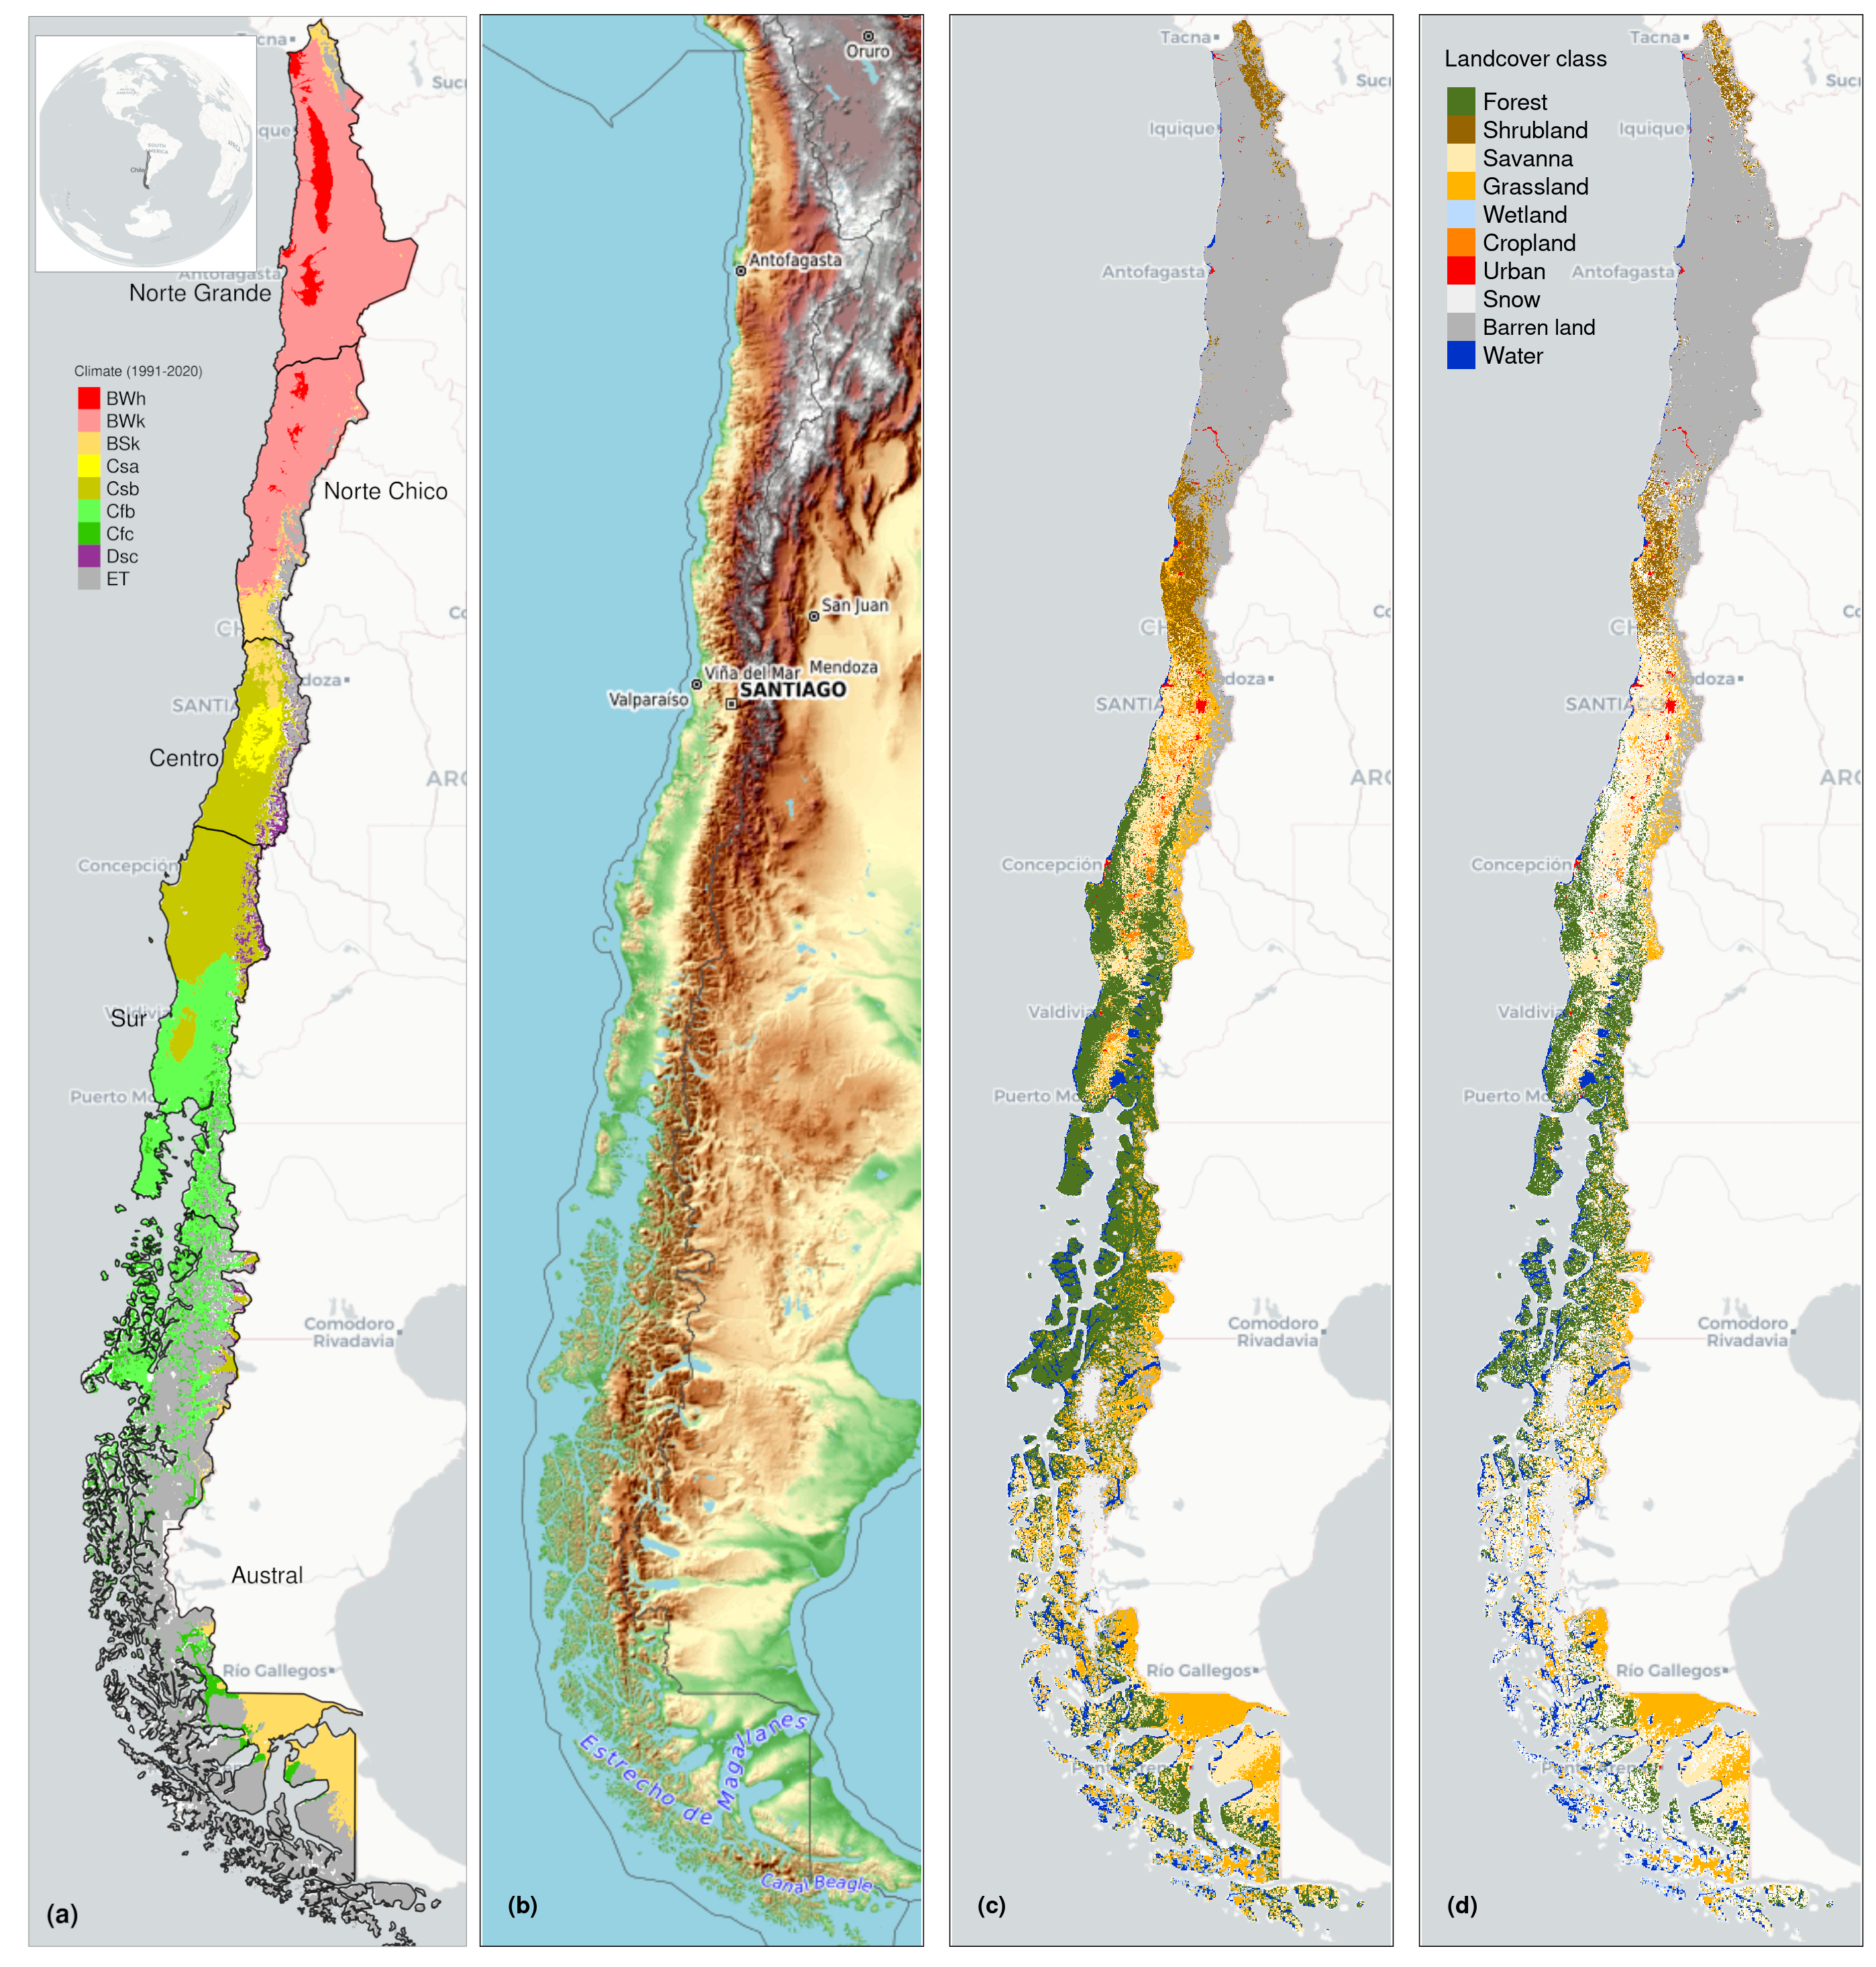
\includegraphics{../output/figs/map_study_con_landcover.png}

}

\caption{\label{fig-studyArea}(a) Chile with the Koppen-Geiger climate
classes and the five macrozones ``Norte Grande'', ``Norte Chico'',
``Centro'', ``Sur'', and ``Austral''. (b) Topography reference map. (c)
land cover classes for 2022. (d) Persistent land cover classes
(\textgreater{} 80\%) for 2001-2022}

\end{figure*}

\hypertarget{materials-and-methods}{%
\section{Materials and Methods}\label{materials-and-methods}}

\hypertarget{data}{%
\subsection{Data}\label{data}}

\hypertarget{gridded-meteorological-and-vegetation-data}{%
\subsubsection{Gridded meteorological and vegetation
data}\label{gridded-meteorological-and-vegetation-data}}

To analyze land cover change, we use the classification scheme by the
IGBP (International Geosphere-Biosphere Programme) from the product
MCD12Q1 collection 6.1 from MODIS. To derive a proxy for vegetation
productivity, we used the Normalized Difference Vegetation Index (NDVI)
from the product MOD13A3 collection 6.1 from MODIS \citep{Didan2015}.
MOD13A3 provides vegetation indices at 1km of spatial resolution and
monthly frequency. The NASA EOSDIS Land Processes Distributed Active
Archive Center (LP DAAC), USGS Earth Resources Observation and Science
(EROS) Center, Sioux Falls, South Dakota, provided the MOD13A3 and
MCD12Q1 from the online Data Pool, accessible at
https://lpdaa.usgs.gov/tools/data-pool/.

\begin{table}[!ht]
\caption{Description of the satellite and reanalysis data used}
\label{tab-desEOD}
\small
\centering
\begin{tabular}{p{0.13\textwidth}cp{0.3\textwidth}p{0.095\textwidth}ccc}
\hline
\multirow{1}{*}{\centering Product} & Sub-product & Variable & Spatial Resolution  & Period & Units & Short Name \\ 
\hline
\multirow{4}{*}{ERA5L} & ~ & Precipitation & \multirow{4}{*}{~0.1°} & \multirow{4}{*}{1981-2023} & mm & P \\ 
         &  & Maximum temperature & ~ & & $°C$ & $T_{max}$ \\ 
         &  & Minimum temperature & ~ & & $°C$ & $T_{min}$ \\ 
         &  & Volumetric Soil Water Content at 1m & ~ & & $m3/m3$ & SM \\ 
ERA5L* & & Atmospheric Evaporative Demand & 0.1° & 1981-2023 & mm & AED \\
        \multirow{2}{*}{MODIS} & MOD13A3.061 & Normalized Difference Vegetation Index & \multirow{2}{*}{~1 km} & 2000-2023 & ~ & NDVI \\ 
         & MCD12Q1.061 & land cover IGBP scheme & & 2001-2022 & ~ & land cover \\ 
\hline
\end{tabular}
{\raggedright *Calculated from maximum and minimum temperatures derived from ERA5L with Eq. \ref{eq-AED}. \par}
\end{table}

For soil moisture, water supply, and water demand variables, we used
ERA5L (ECMWF Reanalysis version 5 over land) \citep{MunozSabater2021}, a
reanalysis dataset that provides the evolution of atmospheric and land
variables since 1950. It has a spatial resolution of 0.1° (9 km), hourly
frequency, and global coverage. We selected the variables for total
precipitation, maximum and minimum temperature at 2 meters, and
volumetric soil water layers between 0 and 100cm of depth (layer 1 to
layer 3). Table \ref{tab-desEOD} shows a summary of the data and its
main characteristics.

\hypertarget{trend-of-short--to-long-term-drought}{%
\subsection{Trend of short- to long-term
drought}\label{trend-of-short--to-long-term-drought}}

\hypertarget{atmospheric-evaporative-demand-aed}{%
\subsubsection{Atmospheric Evaporative Demand
(AED)}\label{atmospheric-evaporative-demand-aed}}

In order to compute the drought indices that use water demand, it is
necessary to first calculate the AED. To do this, we employed the
Hargreaves method \citep{Hargreaves1994, Hargreaves1985} by applying the
following equation:

\begin{equation}\protect\hypertarget{eq-AED}{}{AED = 0.0023\cdot Ra\cdot (T+17.8)\cdot (T_{max}-T_{min})^{0.5}}\label{eq-AED}\end{equation}

where \(Ra\) \((MJ\,m^2\, day^{-1})\) is extraterrestrial radiation;
\(T\), \(T_{max}\), and \(T_{min}\) are mean, maximum, and minimum
temperature \((°C)\) at 2m. For calculating \(Ra\) we used the
coordinate of the latitud of the centroid of each pixel. We chose the
method of Hargreaves to estimate AED because of its simplicity, which
only requires temperatures and extrarrestrial radiation. Also, it has
been recommended over other methods (e.g., Penman-Monteith) when the
access to climatic variables is limited \citep{Vicente-Serrano2014}.

\hypertarget{non-parametric-calculation-of-drought-indices}{%
\subsubsection{Non-parametric calculation of drought
indices}\label{non-parametric-calculation-of-drought-indices}}

To derive the drought indices of water supply and demand, soil moisture,
and vegetation (i.e., the proxy of productivity), we used the ERA5L
dataset and the MODIS product, with a monthly frequency for 1981--2023
and 2000--2023, respectively.

The dought indices correspond to a historical anomaly with regard to a
variable (e.g., meteorological, vegetation, or soil moisture). To
account for the anomaly, the common practice is to derive it following a
statistical parametric methodology in which it is assumed that the
statistical distribution of the data is known (\citet{Heim2002}). A
wrong decision is usually the highest source of uncertainty
(\citet{Laimighofer2022}). In the case of Chile, due to its high degree
of climatic variability, it is complex to choose a proper distribution
without previous research. Here, we follow a non-parametric methodology
for the calculation of the drought indices, in a similar manner as the
framework proposed by \citet{Farahmand2015};
\citet{Hobbins2016};\citet{McEvoy2016}.

For the purpose of monitoring water supply drought, we used the
well-known Standardized Precipitation Index (SPI), which the World
Meteorological Organization (WMO) recommended. The SPI solely relies on
precipitation data. Also, it has been used worldwide for the study of
drought, including in Chile (\citet{Garreaud2017};
\citet{Zambrano2017}). The primary cause of drought is precipitation
anomalies, and temperature usually makes it worse \citep{Luo2017}.
Nowadays, there is an increase in attention toward using water demand
separately to monitor droughts. (\citet{Vicente-Serrano2020};
\citet{Noguera2022}). Thus, to evaluate water demand, we chose the
Evaporative Demand Drought Index (EDDI), developed by
\citet{Hobbins2016} and \citet{McEvoy2016}, which is based on the AED.
EDDI is currently used for monitoring drought in the United States
(https://psl.noaa.gov/eddi/). In our case, we used only temperature for
AED, a difference from the original formulation of EDDI, which also
considered wind besides temperature. To consider the combined effect of
water supply and demand, we selected the SPEI, which corresponds to a
balance between precipitation and AED. \citet{Vicente-Serrano2010}
proposed the SPEI, and it has improved the SPI by incorporating
temperature for drought monitoring. For SPEI, an auxiliary variable D =
P-AED is calculated. Soil moisture is the main driver of vegetation
productivity, particularly in semi-arid regions (\citet{Li2022}). Hence,
for soil water drought, we used the SSI (Standardized Soil Moisture
Index) \citep{Hao2013, AghaKouchak2014} which is a multi-scale index
similar to SPI, SPEI, and EDDI. In our case, for the SSI, we used the
average soil moisture from ERA5L at 1m depth. Finally, for the proxy of
productivity, we used the zcNDVI proposed by \citet{Zambrano2018} which
will be derived from the NDVI retrieved from MOD13A1.

To derive the drought indices, first we must calculate the sum of the
variables with regard to the time scale (s). In this case, for
generalization purposes, we will use \(V\), referring to variables
\(P\), \(AED\), \(D\), \(NDVI\), and \(SM\) (Table \ref{tab-desEOD}). We
cumulated each \(V\) over the time series of \(n\) values (months), and
for the time scales \(s\):

\begin{equation}\protect\hypertarget{eq-sumvar}{}{A_{si} = \sum_{i=n-s-i+2}^{n-i+1} V_i\,\, \forall\, i\geq n-s+1  }\label{eq-sumvar}\end{equation}

The \(A_{si}\) corresponds to a moving window (convolution) that sums
the variable for time scales \(s\) from the last month, month by month,
until the first month in which it could sum for \(s\) months. Once the
variable is cumulated over time for the scale \(s\). Thus, the
empirically derived probabilities are obtained through an inverse normal
approximation \citep{Abramowitz1968}. Then, we used the empirical Tukey
plotting position \citep{Wilks2011} over \(A_i\) to derive the
\(P(a_i)\) probabilities across a period of interest:

\begin{equation}\protect\hypertarget{eq-probPai}{}{P(A_i) = \frac{i-0.33}{n+0.33'}}\label{eq-probPai}\end{equation}

The drought indices \(SPI\), \(SPEI\), \(EDDI\), \(SSI\), and \(zcNDVI\)
are obtained following the inverse normal approximation:

\begin{equation}\protect\hypertarget{eq-DI}{}{DI(A_i) = W - \frac{C_0+C_1\cdot W + c_2 \cdot W^2}{1+d_1\cdot W +d_2\cdot W^2 +d_3\cdot W^3}}\label{eq-DI}\end{equation}

\(DI\) is referring to the drought index calculated for the variable
\(V\). The values for the constats are: \(C_0 = 2.515517\),
\(C_1 = 0.802853\), \(C_2 = 0.010328\), \(d_1 = 1.432788\),
\(d_2 = 0.189269\), and \(d3 = 0.001308\). For \(P(A) \leq 0.5\),
W=\(\sqrt{-2\cdot ln(P(A_i))}\) , and for \(P(A_i) > 0.5\), replace
\(P(A_i)\) with \(1-P(A_i)\) and reverse the sign of \(DI(A_i)\).

The drought indices were calculated for time scales of 1, 3, 6, 12, 24,
and 36 months at a monthly frequency for 1981--2023 in order to be used
for short- to long-term evaluation of drought. In the case of the proxy
of vegetation productivity (zcNDVI) it was calculated for a time scale
of six months at monthly frequency for 2000--2023. For zcNDVI, we test
time scales of 1, 3, 6, and 12 months; we choose to use six months
because that shows a more robust representation of vegetation
productivity due to the seasonality of vegetation in Chile.

\hypertarget{trend-of-drought-indices}{%
\subsubsection{Trend of drought
indices}\label{trend-of-drought-indices}}

To estimate if there are significant positive or negative trends for the
drought indices, we used the non-parametric test of Mann-Kendall
\citep{Kendall1975}. To determine the magnitude of the trend, we used
Sen's slope \citep{Sen1968}. Some of the advantages of applying this
methodology are that the Sen's slope is not affected by outliers as
regular regression does, and it is a non-parametric method that is not
influenced by the distribution of the data. We applied Mann-Kendall to
see if the trend was significant and Sen's slope to estimate the
magnitude of the trend. We did this to the six time scales from 1981 to
2023 (monthly frequency) and the indices SPI, EDDI, SPEI, and SSI. Thus,
we have trends per index and time scale (24 in total). Then, we
extracted the trend aggregated by macrozone and per land cover persitent
macroclasses.

\hypertarget{interaction-of-land-cover-and-drought}{%
\subsection{Interaction of land cover and
drought}\label{interaction-of-land-cover-and-drought}}

\hypertarget{land-cover-change}{%
\subsubsection{Land cover change}\label{land-cover-change}}

To analyze the land cover change, we use the IGBP scheme from the
MCD12Q1 collection 6.1 from MODIS. \citet{Zambrano2018} and
\citet{Fuentes2021} have previously used this product for studies of
drought and land cover in Chile. The MCD12Q1 has a yearly frequency from
2001 to 2022. The IGBP defines 17 classes; from these, we regrouped into
ten macroclasses, as follows: classes 1-4 to forest, 5-7 to shrublands,
8-9 to savannas, 10 as grasslands, 11 as wetlands, 12 and 14 to
croplands, 13 as urban, 15 as snow and ice, 16 as barren, and 17 to
water bodies. Thus, we have a land cover raster time series with the ten
macroclasses for 2001 and 2023. We validate the land cover macroclasses
regarding a highly detailed (30 m of spatial resolution) land cover map
made for Chile by \citet{Zhao2016} for 2013-2014. Our results showed a
global accuracy of \textasciitilde0.82 and a F1 score of
\textasciitilde0.66. Section S2 in the Supplementary Material shows the
procedure for validation.

Climate, vegetation development, seasonality, and changes in vegetation
type all have an impact on the time series of NDVI. In this study, we
want to examine the variation in vegetation productivity across various
land cover types and how water demand, water supply, and soil moisture
affect it. In order to avoid changes due to a change in the land cover
type that will wrongly impact NDVI, we developed a persistence mask for
land cover for 2001--2022. Thereby, we reduce an important source of
variation on a regional scale. Therefore, we generated a raster mask for
IGBP MODIS per pixel using macroclasses that remained unchanged for at
least 80\% of the years (2001--2022). This enabled us to identify
regions where the land cover macroclasses are persistent. We calculated
the surface occupied per land cover class into the five macrozones
(``Norte Grande'' to ``Austral'') per year for 2001--2023. After that,
we calculated the trend's change in surface per type. We used the Sen'
slope \citep{Sen1968} based on Mann-Kendall \citep{Kendall1975}.

\hypertarget{relationship-between-land-cover-and-drought-trends}{%
\subsubsection{Relationship between land cover and drought
trends}\label{relationship-between-land-cover-and-drought-trends}}

We wanted to explore the relationship between the trend in land cover
classes and the trend in the drought indices. For this purpose, in order
to have more representative results, we conducted the analysis over
sub-basins within continental Chile. We use 469 basins, which have a
surface area between 0.0746 and 24,000 (\(km^2\)), and a median area of
1,249 (\(km^2\)). For each basin, we calculate the relative trend per
land cover type, considering the proportion of the type relative to the
total surface of the basin. Then, we extracted per basin the average
trend of the drought indices SPI, SPEI, EDDI, SSI, and all their time
scales 1, 3, 6, 12, 24, and 36. Also, we extracted the average trend in
the proxy of vegetation productivity (zcNDVI). We wanted to analyze
which drought indices and time scales have a major impact on changes in
land cover type.

We have 25 predictors, which are drought indices and vegetation
productivity. We analyzed the 25 predictors per type of landcover. For
the analysis, we selected the method of random forest (\citet{Ho1995}).
Because it allows to find no linear relationship, it reduces overfitting
and can derive the feature importance, which helps for a better
understanding of the relationships. The importance of the variable is
calculated by permuting out-of-bag (OOB) data per tree and calculating
the mean standard error in the OOB. Then the same is done after
permuting each predictor variable. Random forest uses multiple decision
trees and allows for classification and regression.

We analyzed the 25 predictors per type of landcover, thus running six
models. We used random forests for regression and trained 1000 forests.
For more reliable results for the important variables, we resampled by
creating ten folds, running a random forest per fold, and calculating
the r-squared (rsq), root mean square error (RMSE), and variable
importance ten times.

\hypertarget{drought-impacts-on-vegetation-productivity}{%
\subsection{Drought impacts on vegetation
productivity}\label{drought-impacts-on-vegetation-productivity}}

We analyzed the trend of vegetation productivity over the unchanged land
cover macroclasses. This way, we tried to reduce the noise in the
vegetation due to a change in land cover from year to year. To achieve
this, we will use the persistent mask of land cover macroclasses, which
are the types that remain more than 80\% of the time for 2001--2022. We
used this to evaluate the trend in zcNDVI per land cover class and
macrozone.

We examine the drought indices of water demand, water supply, soil
moisture, and their connection with vegetation productivity to
investigate two main questions: i) whether short-term or long-term time
scales have a greater impact on vegetation across Chile and its specific
regions; and ii) the spatial variation in the strength of the
correlation between the variables and time scales.~ Then, we will
summarize for each land cover class and macrozone. Thus, we will be able
to advance in understanding how climate is affecting vegetation,
considering the impact on the five macroclasses of vegetation: forest,
cropland, grassland, savanna, and shrubland.

We conducted an analysis on the linear correlation between the indices
SPI, SPEI, EDDI, and SSI over time periods of 1, 3, 6, 12, 24, and 36
months, and zcNDVI. The objective is to determine the impact of soil
moisture and water demand and supply on vegetation productivity. We used
a method similar to that used by \citet{Meroni2017} which compared the
SPI with the cumulative FAPAR (Fraction of Absorbed Photosynthetically
Active Radiation). A pixel-to-pixel linear correlation analysis was
performed for each index within the persistent mask of land cover
macroclasses. To begin, the Pearson coefficient of correlation is
computed for each of the six time scales. A significant time scale is
identified as the one that attains the highest correlation (p
\textless{} 0.05). Subsequently, the Pearson correlation coefficient
corresponding to the time scales at which the value peaked was
extracted. As a result, for each index, we generated two raster maps: 1)
containing the raster with values of the time scales that reached the
maximum correlation, and 2) having the value of the correlation
obtained.

\hypertarget{software-and-packages-used}{%
\subsection{Software and packages
used}\label{software-and-packages-used}}

For the downloading, processing, and analysis of the spatio-temporal
data, we used the open source software for statistical computing and
graphics, \texttt{R} \citep{R2023}. For downloading ERA5L, we used the
\texttt{\{ecmwfr\}} package \citep{Hufkens2019}. For processing raster
data, we used \texttt{\{terra\}} \citep{Hijmans2023} and
\texttt{\{stars\}} \citep{Pebesma2023}. For managing vectorial data, we
used \texttt{\{sf\}} \citep{Pebesma2018}. For the calculation of AED, we
used \texttt{\{SPEI\}} \citep{Bergueria2023}. For mapping, we use
\{tmap\} \citep{Tennekes2018}. For data analysis, the suite
\{tidyverse\} \citep{Wickham2019} was used.

\hypertarget{results}{%
\section{Results}\label{results}}

\hypertarget{trend-of-short--to-long-term-drought-1}{%
\subsection{Trend of short- to long-term
drought}\label{trend-of-short--to-long-term-drought-1}}

Figure~\ref{fig-trendDI} shows the spatial variation of the trend for
the drought indices from short- to long-term scales. SPI and SPEI have a
decreasing trend from ``Norte Chico'' to ``Sur.'' However, there is an
increasing trend in ``Austral.'' The degree of the trend is stronger at
higher time scales. The SSI indicates that in ``Norte Grande,'' there
are surfaces that have increased in the soutwest part and in the
northeast have decreased, and is shown for all time scales. Similar to
SPI and SPEI, SSI decreases at higher time scales. EDDI showed a
positive trend for the whole of continental Chile, with a higher trend
toward the north and a descending gradient toward the south. The degree
of trend increases at higher time scales.

\blandscape

\begin{figure}

\begin{minipage}[t]{0.50\linewidth}

{\centering 

\raisebox{-\height}{

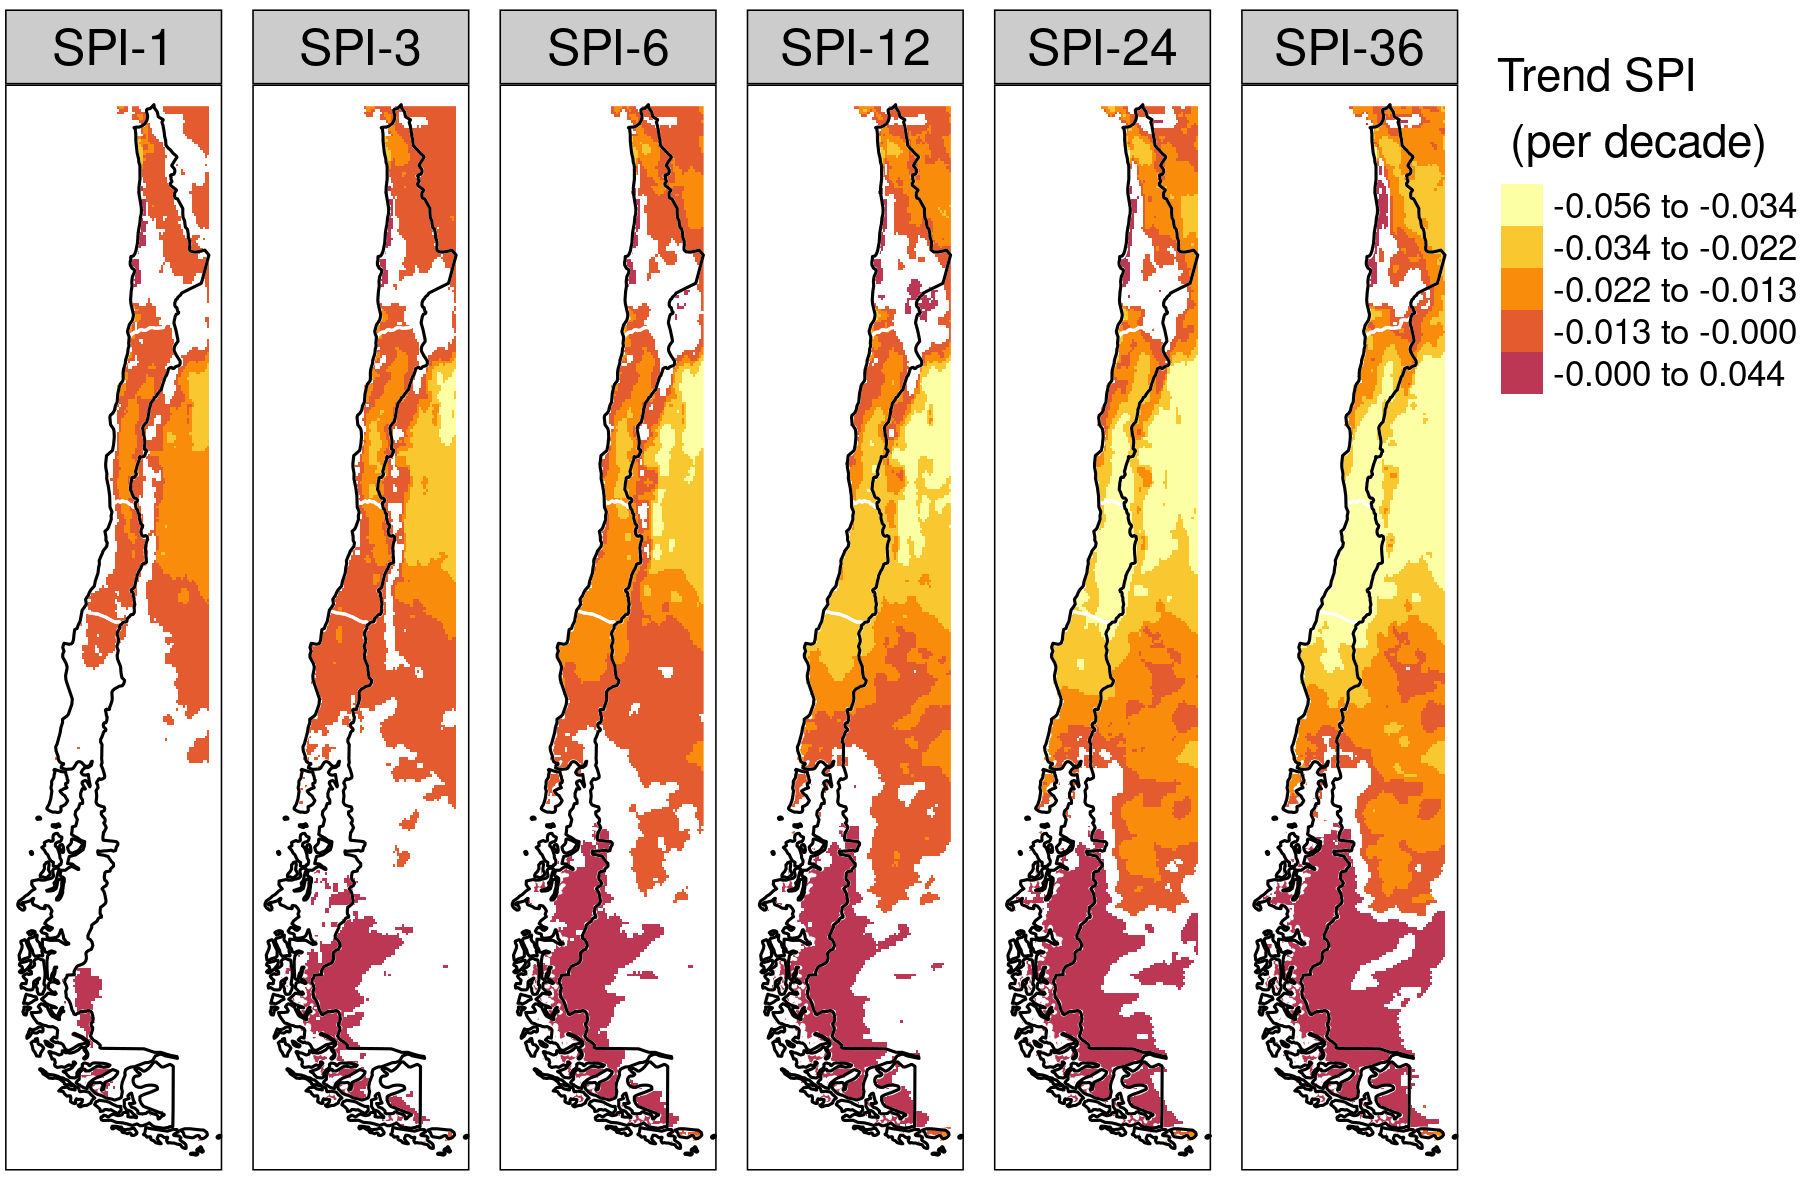
\includegraphics{../output/figs/trend_raster_SPI_1981-2023.png}

}

}

\subcaption{\label{fig-trendDI-1}SPI (Standardized Precipitation Index)}
\end{minipage}%
%
\begin{minipage}[t]{0.50\linewidth}

{\centering 

\raisebox{-\height}{

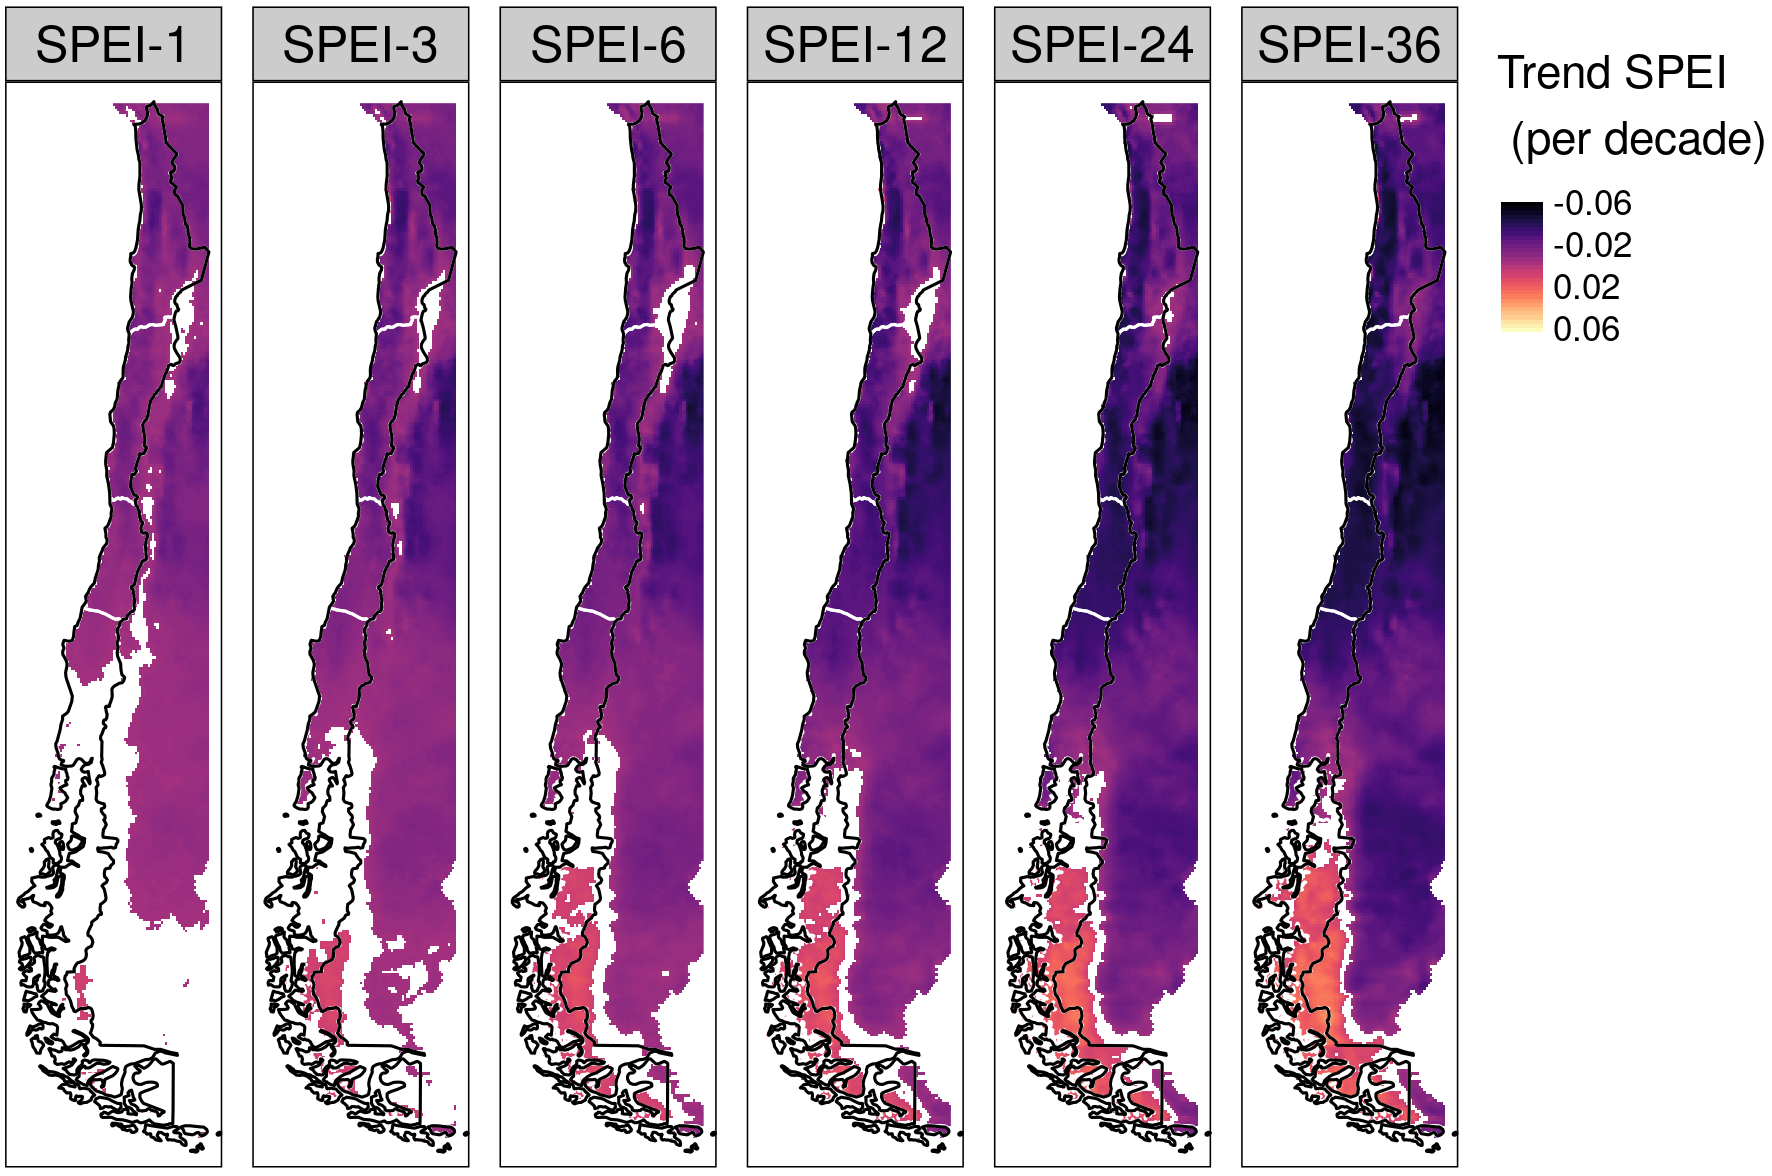
\includegraphics{../output/figs/trend_raster_SPEI_1981-2023.png}

}

}

\subcaption{\label{fig-trendDI-2}SPEI (Standardized Precipitation
Evapotranspiration Index)}
\end{minipage}%
\newline
\begin{minipage}[t]{0.50\linewidth}

{\centering 

\raisebox{-\height}{

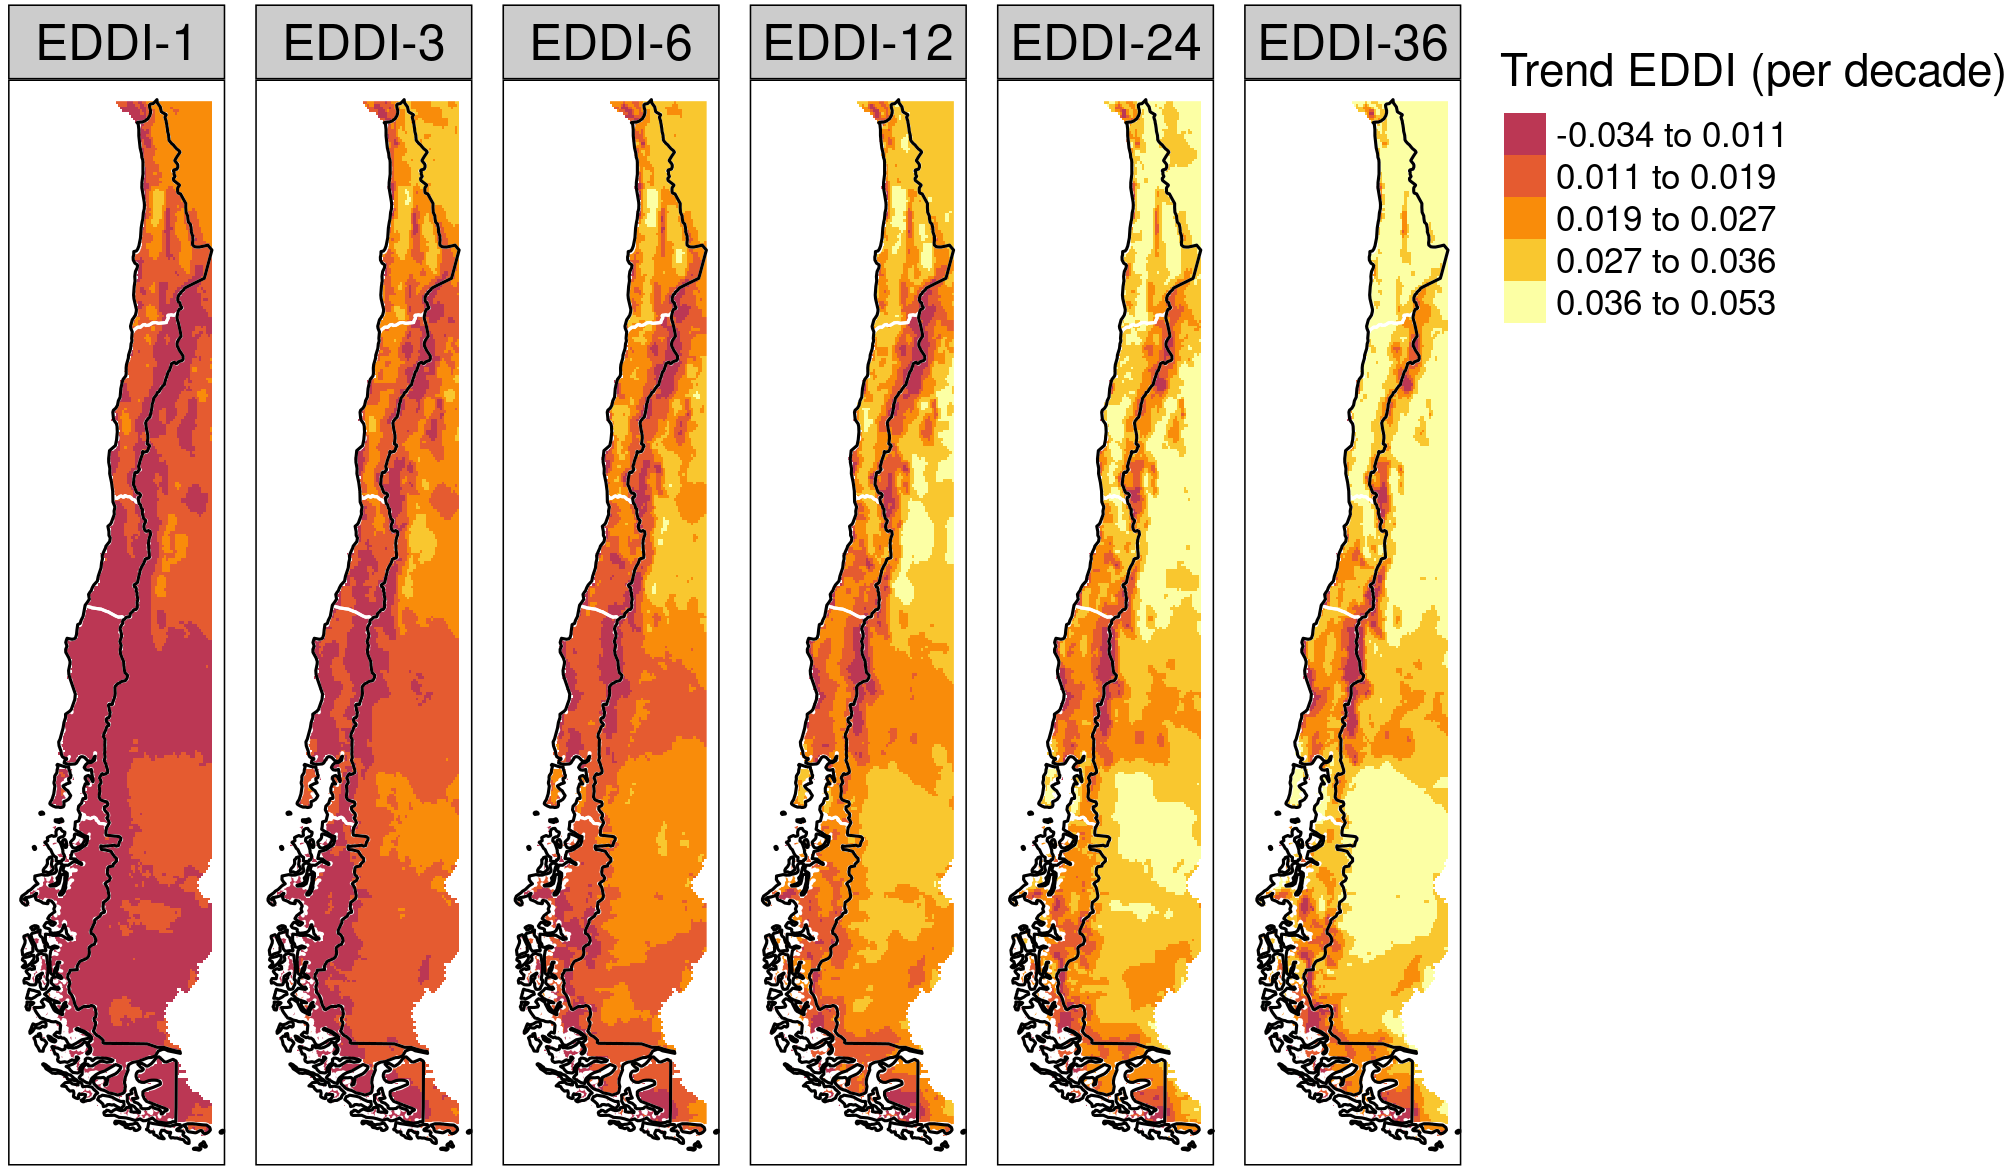
\includegraphics{../output/figs/trend_raster_EDDI_1981-2023.png}

}

}

\subcaption{\label{fig-trendDI-3}EDDI (Evaporative Demand Drought
Index)}
\end{minipage}%
%
\begin{minipage}[t]{0.50\linewidth}

{\centering 

\raisebox{-\height}{

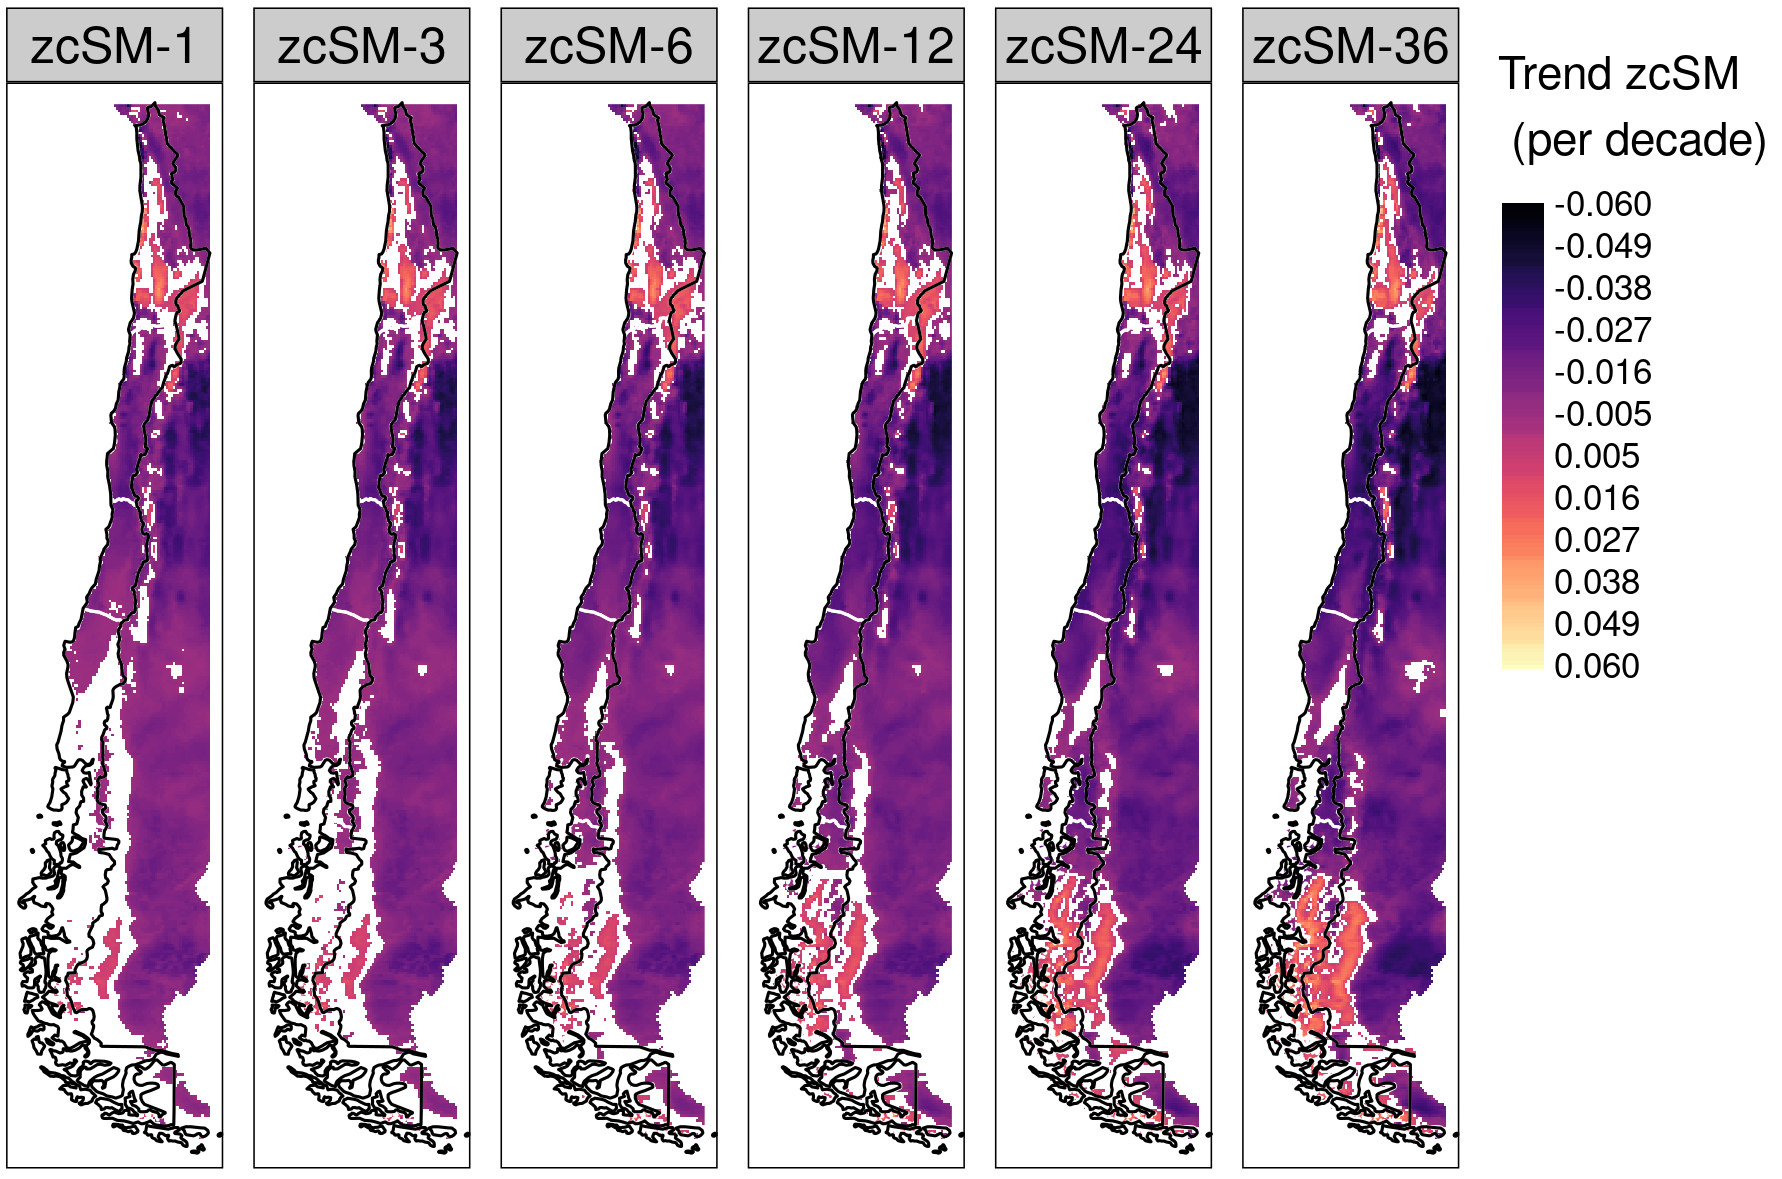
\includegraphics{../output/figs/trend_raster_zcSM_1981-2023.png}

}

}

\subcaption{\label{fig-trendDI-4}SSMI (Standardized Soil Moisture
Index)}
\end{minipage}%

\caption{\label{fig-trendDI}Linear trend of the drought index (*) at
time scales of 1, 3, 6, 12, 24, and 36 months for 1981-2023}

\end{figure}

\elandscape

\begin{figure}[!ht]

{\centering 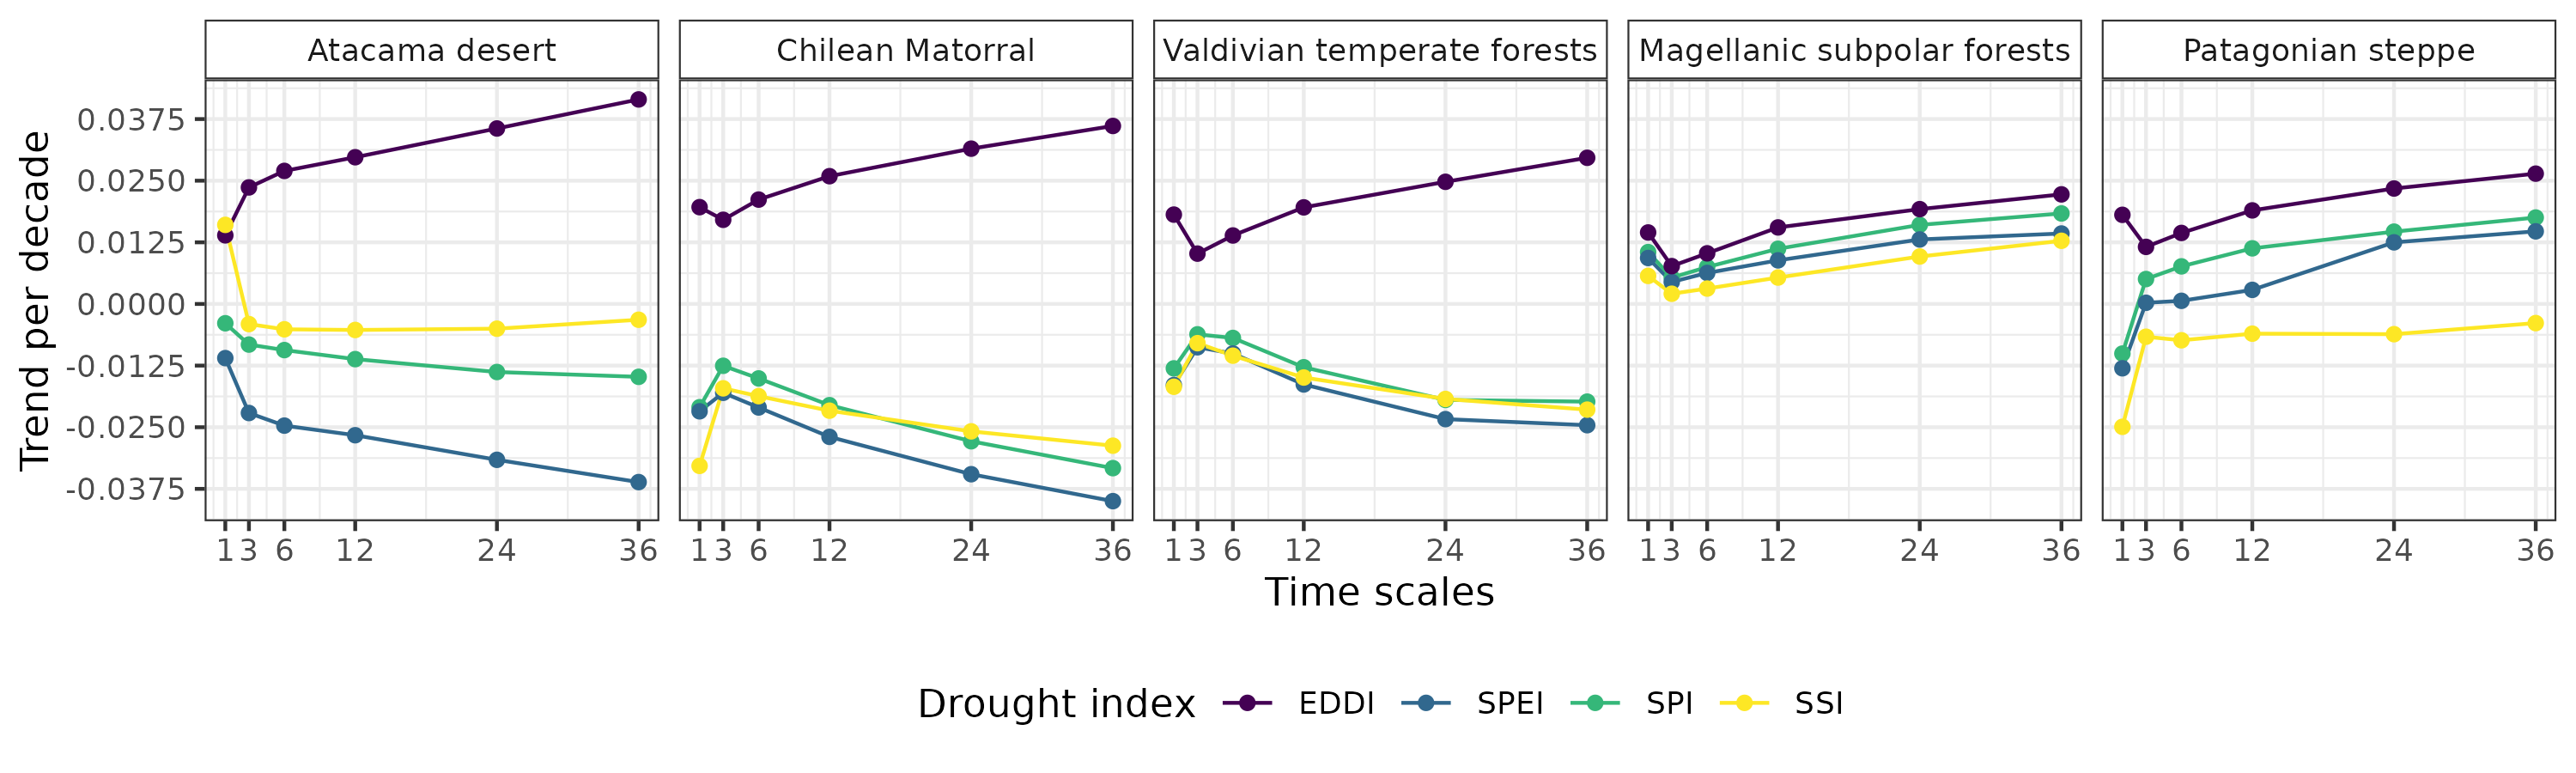
\includegraphics{../output/figs/trend_macrozone_drought_indices.png}

}

\caption{\label{fig-trendDIMacro}Trend per decade for the drought
indices SPI, EDDI, SPEI, and SSI aggregated by macrozone.}

\end{figure}

In Figure~\ref{fig-trendDIMacro}, the averaged aggregation per
macrozone, drought index, and time scale are shown. The macrozones that
have the lowest trend are ``Norte Chico'' and ``Centro,'' where the SPI,
SPEI, and SSI show that it decreases at longer time scales. Potentially
explained due to the prolonged reduction in precipitation that has
affected the hydrological system in Chile. At 36 months, it reaches
trends between -0.03 and -0.04 (z-score) per decade for SPI, SPEI, and
SSI. For ``Sur,'' the behavior is similar, decreasing at longer scales
and having between -0.016 and -0.025 per decade for SPI, SPEI, and SSI.
``Norte Grande'' has the highest trend at 36 months for EDDI (0.042 per
decade), and ``Centro'' has the lowest for SPI and SPEI. In ``Norte
Grande'' and ``Norte Chico,'' which are in a semi-arid climate, it is
evident that the EDDI has an effect on the difference between the SPI
and SPEI index, which is not seen in the other macrozones. Contrary to
the other macrozones, ``Austral'' showed an increase in all indices,
being the highest for EDDI at 36 months (0.025) and the lowest for SSI,
which shows only a minor increase in the trend.

\hypertarget{interaction-of-land-cover-and-drought-1}{%
\subsubsection{Interaction of land cover and
drought}\label{interaction-of-land-cover-and-drought-1}}

\hypertarget{land-cover-change-1}{%
\subsection{Land cover change}\label{land-cover-change-1}}

\begin{table}[!ht]
\caption{Surface of the land cover class that persist during 2001-2022}
\label{tab-landcoverSurf}
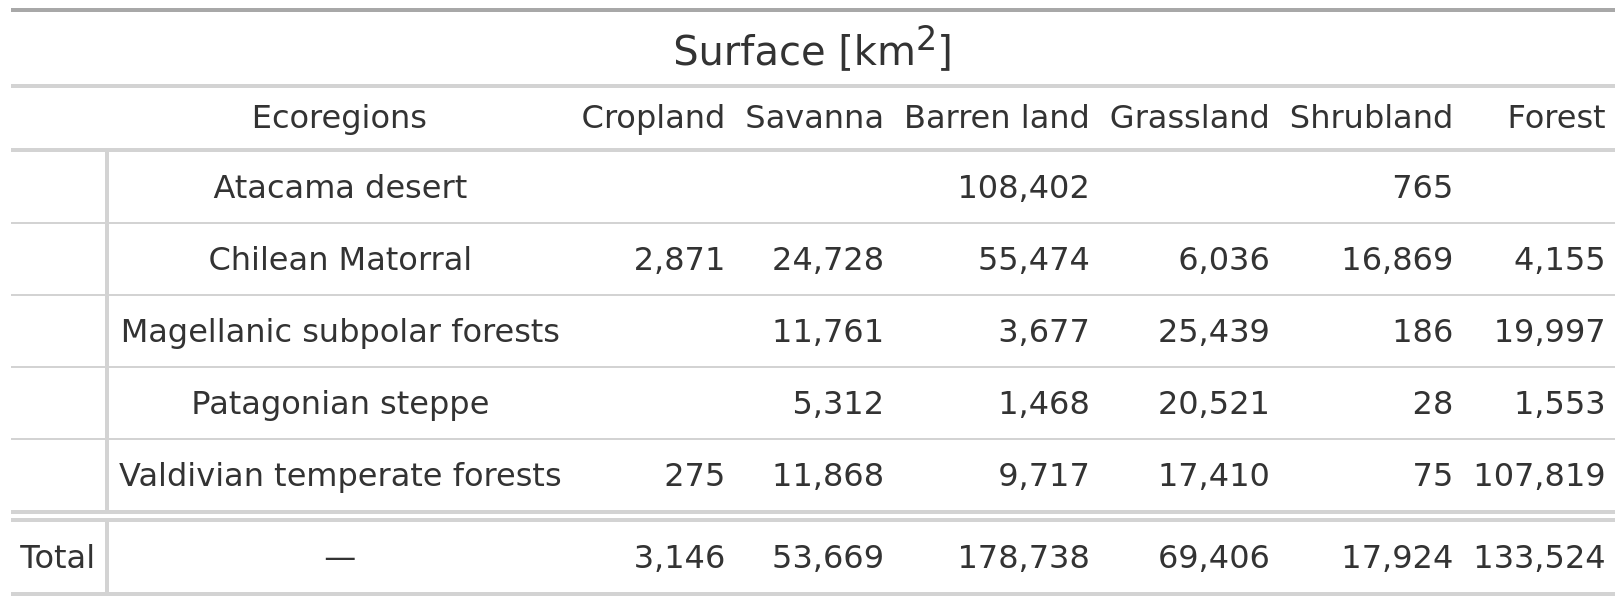
\includegraphics[width = .5\textwidth]{../output/figs/table_surface_landcover_macrozone.png}
\end{table}

\begin{figure}[!ht]

{\centering 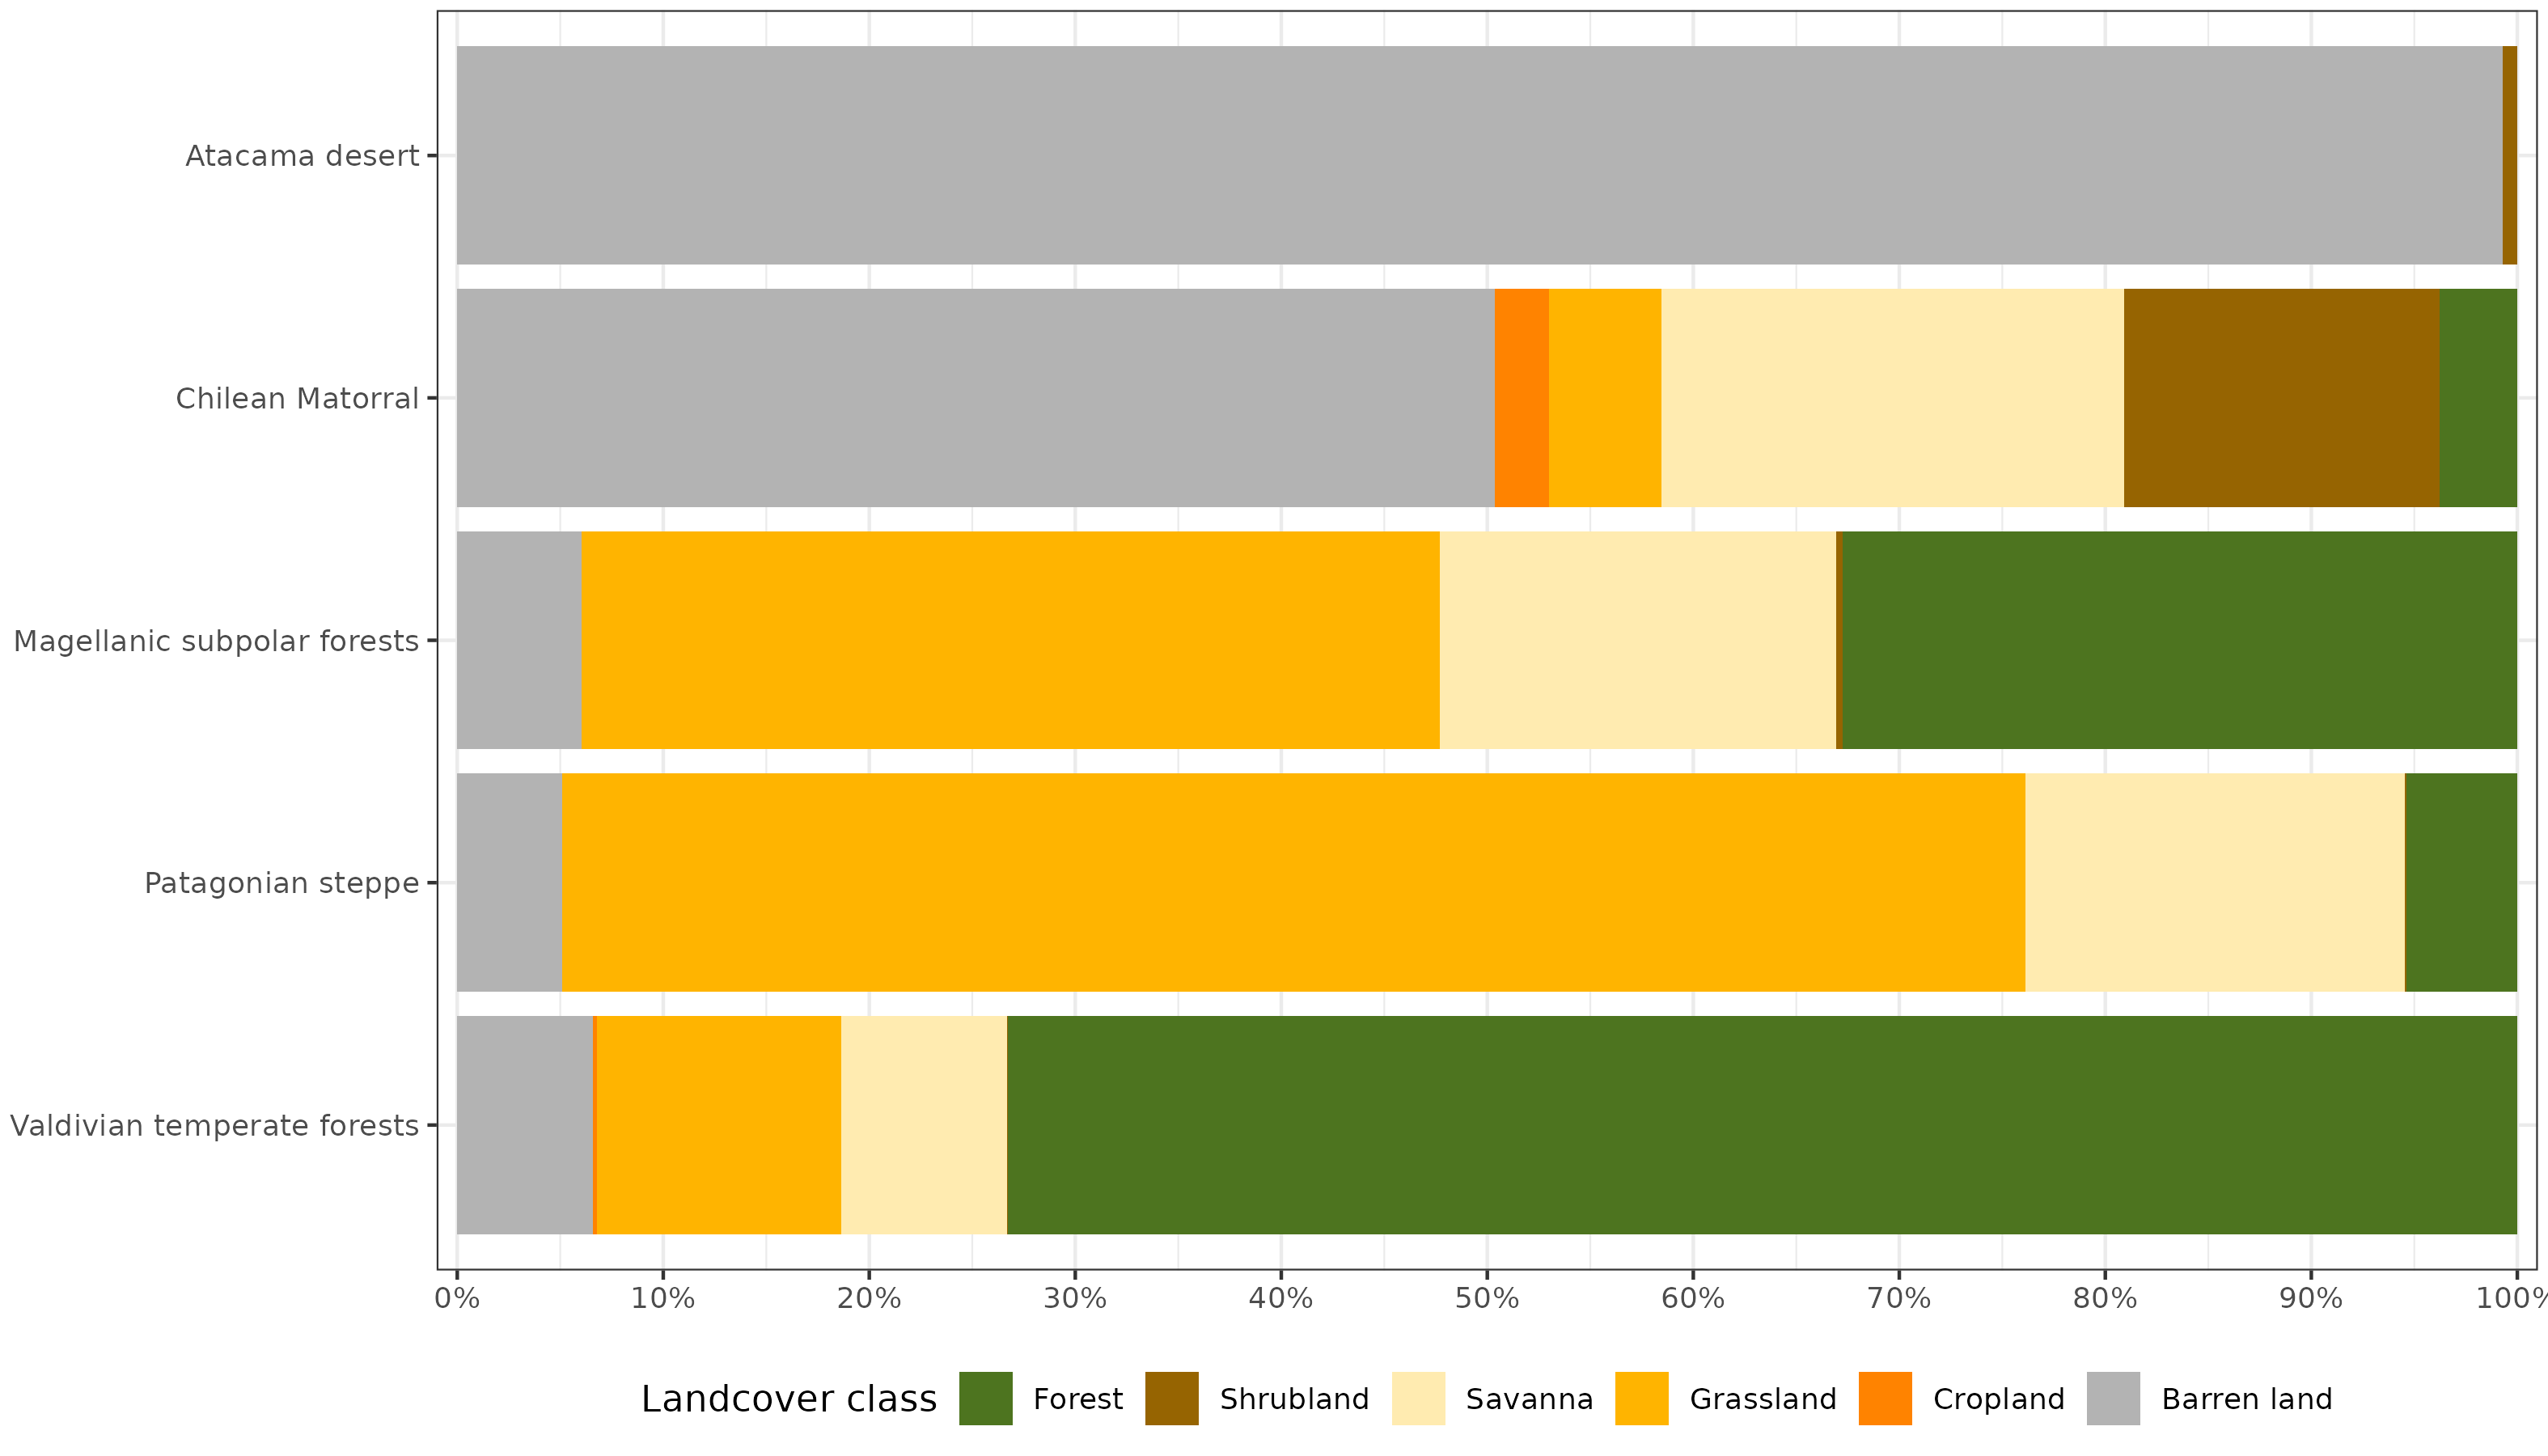
\includegraphics{../output/figs/LC_pers80_per_macrozone.png}

}

\caption{\label{fig-LCprop}Proportion of land cover class from the
persistent land cover for 2001-2022 (\textgreater80\%) per macrozone}

\end{figure}

For vegetation, we obtained and use hereafter five macroclasses of land
cover from IGBP MODIS: forest, shrubland, savanna, grassland, and
croplands. Figure~\ref{fig-studyArea}c shows the spatial distribution of
the macroclasses through Chile for the year 2022.
Figure~\ref{fig-studyArea}d shows the macroclasses of land cover
persistance (80\%) during 2021--2022, respectively (Table
\ref{tab-landcoverSurf}). Within continental Chile, barren land is the
land cover class with the highest surface area (277,870 km2). The
largest type of vegetation, with 137,085 km2, is forest. Grassland
(74,247 km2), savanna (55,206 km2), shrubland (25,341 km2), and cropland
(3,146 km2) are the other types (Table \ref{tab-landcoverSurf}). The
macrozones with major changes for 2001--2022 were ``Centro,'' ``Sur,''
and ``Austral,'' with 36\%, 31\%, and 34\% of their surface changing the
type of land cover, respectively (Figure~\ref{fig-studyArea} and Table
\ref{tab-landcoverTrend}). Figure~\ref{fig-LCprop} shows the summary of
the proportion of surface per land cover class and macrozone, derived
from the persistance mask over continental Chile.

\begin{table}[!ht]
\caption{The value of Sen's slope trend next to the time-series plot of surface per land cover class (IGBP MCD12Q1.016) for 2001–2022 through Central Chile. Values of zero indicate that there was not a significant trend. Red dots on the plots indicate the maximum and minimum values of surface.}
\label{tab-landcoverTrend}
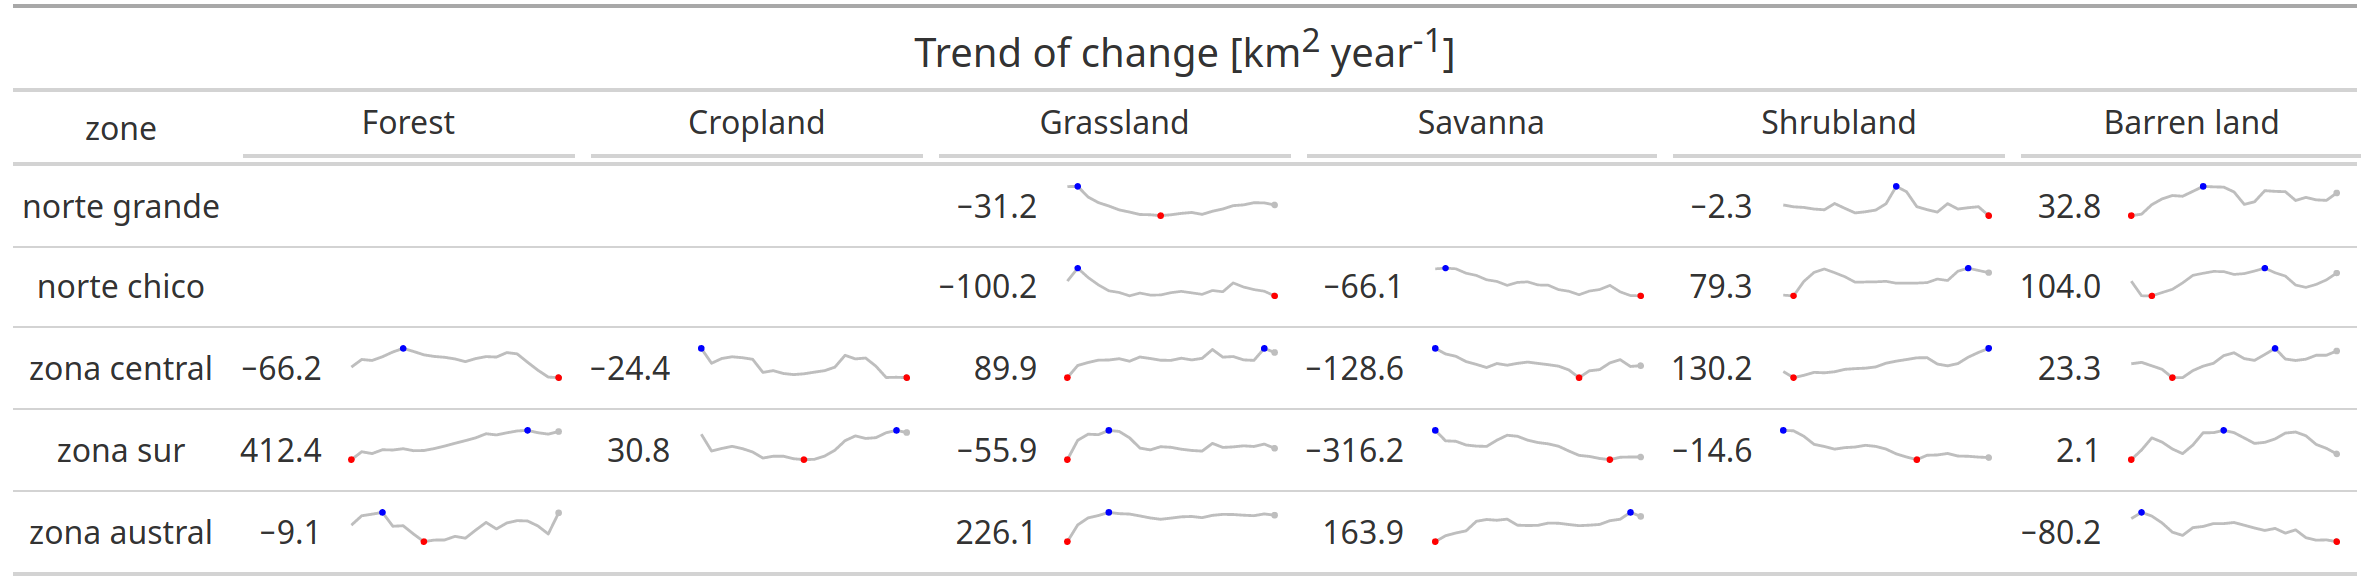
\includegraphics[]{../output/figs/table_var_landcover_macro.png}
\end{table}

The ``Norte Chico'' shows an increase in barren land of 111
\(km^2 yr^{-1}\) and a reduction in the class savanna of 70
\(km^2 yr^{-1}\). In the ``Centro'' and ``Sur,'' there are changes with
an important reduction in savanna (136 to 318 \(km^2 yr^{-1}\) ), and an
increase in shrubland and grassland. Showing a change for more dense
vegetation types. It appears to be a shift in the area cultivated
(croplands) from the ``Centro'' to the ``Sur.'' Also, there is a high
increase in forest (397 \(km^2 yr^{-1}\) ) in the ``Sur,'' replacing the
savanna lost (Table \ref{tab-landcoverTrend}).

\hypertarget{relationship-between-drought-indices-and-land-cover-change}{%
\subsubsection{Relationship between drought indices and land cover
change}\label{relationship-between-drought-indices-and-land-cover-change}}

According to Table \ref{tab-landcoverTrendRF}, the trends in drought
indices reach an r-squared between 0.32 and 0.39 for the types of
forest, grassland, savanna, shrubland, and barren land. It is more
likely that short- and medium-term increases in AED (EDDI-6 and EDDI-12)
and short-term precipitation deficits (SPI-6 and SPEI-6) contributed to
changes in grassland and bare land. The short-term increase of AED
(EDDI-3 and EDDI-6) and the longer duration of the precipitation deficit
(SPI-24, SPI-36, and SPEI-36) most likely contribute to the changes in
shrubland. The changes in savanna are associated with a short- and
long-term increase in AED and a three-year precipitation deficit
(SPI-36). The increase in cumulative AED from 12 to 36 months is the
strongest associated variable that contributes to changes in forests,
followed by the reduction of soil moisture over six and 36 months. More
details about the results of the variable importance can be found in the
supplementary material in Section S3.

\begin{table}[!ht]
\caption{The five most important trends of drought indices in estimating the landcover trend per land cover type and the r-squared (rsq) reached by each random forest model.}
\label{tab-landcoverTrendRF}
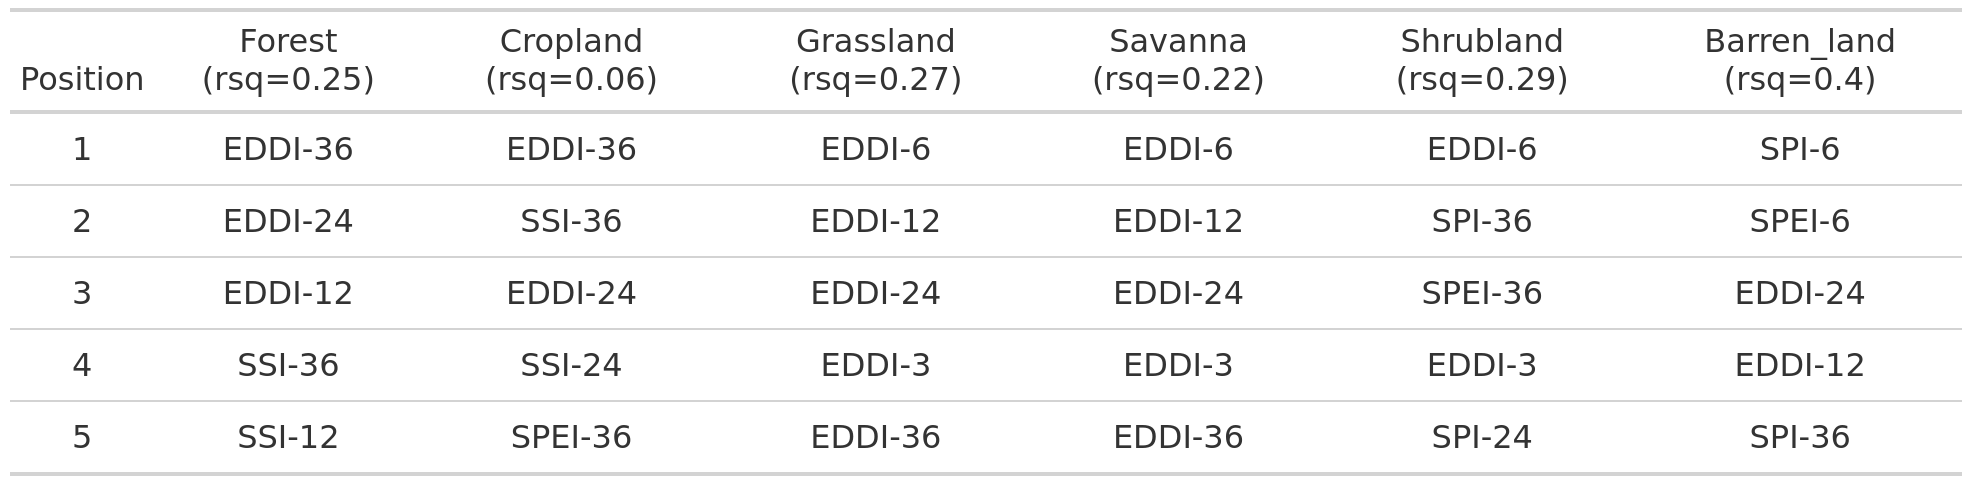
\includegraphics[]{../output/figs/table_importance_trends_landcover_vs_drought.png}
\end{table}

\begin{figure}[!ht]

{\centering 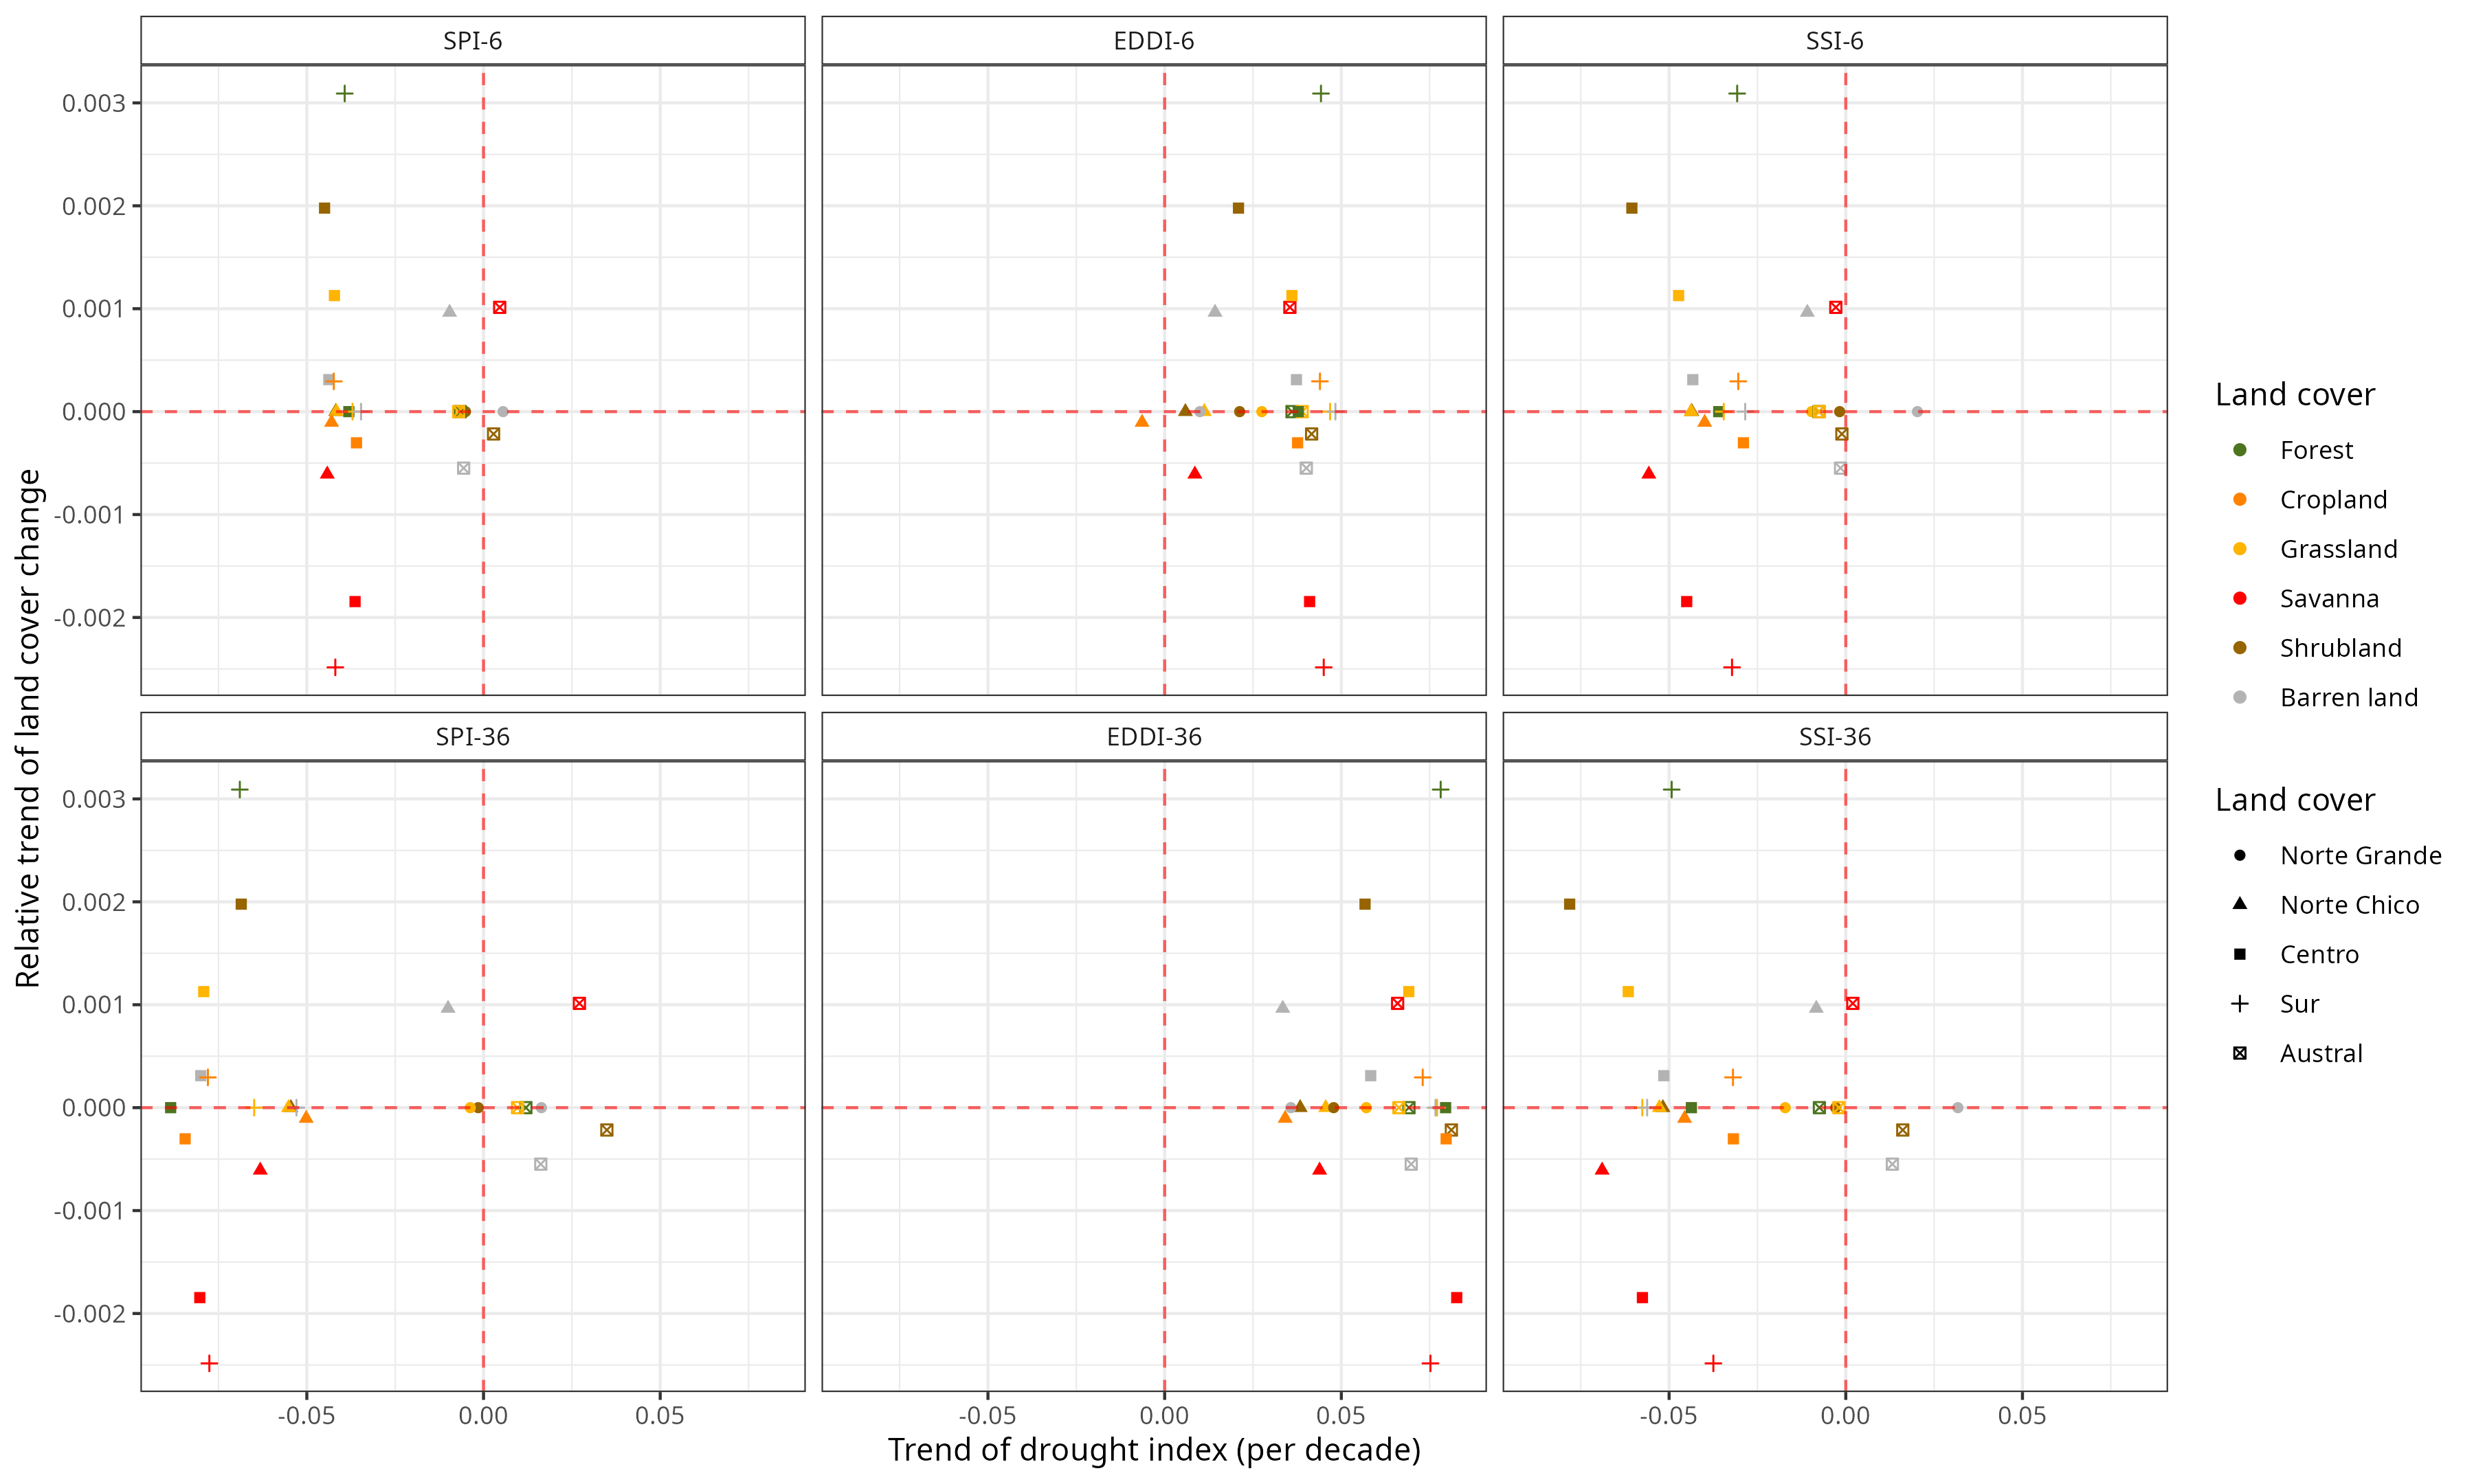
\includegraphics{../output/figs/points_landcover_drought_indices_trend_and_time_scale.png}

}

\caption{\label{fig-TrendsLandDrought}Relationship between the trend in
land cover change (y-axis) and the trend in drought indices (x-axis) for
the five macrozones. Vertical panels correspond to 1, 3, 6, 12, 24, and
36 months of the time scale by drought index. Horizontal panels show
each drought index}

\end{figure}

We study the connection between the SPI, EDDI, and SSI drought indices
and changes in land cover in Figure~\ref{fig-TrendsLandDrought}. To do
this, we compare the relative changes in land cover (in terms of the
total surface area per land cover type and macrozone) over six and
thirty-six months. Figure~\ref{fig-TrendsLandDrought} shows that the
forest in the ``Sur,'' shrubland and grassland in ``Centro,'' barren
land in ``Norte Chico,'' and savanna in ``Austral'' showed an increase
in the surface of landcover associated with an increase in EDDI. Savanna
in ``Centro,'' ``Sur,'' and ``Norte Chico'' decreases with the increase
in EDDI. The SPI and SSI showed similar behavior regarding the trend in
land cover type. A decrease in SPI and SSI is associated with an
increase in the surface in shurubland and grassland in ``Centro,''
forest in ``Sur,'' and barren land in ``Norte Chico,'' as well as a
decrease trend in savanna in ``Norte Chico,'' ``Centro,'' and ``Sur.''

\hypertarget{drought-impacts-on-vegetation-productivity-within-land-cover}{%
\subsection{Drought impacts on vegetation productivity within land
cover}\label{drought-impacts-on-vegetation-productivity-within-land-cover}}

\hypertarget{vegetation-productivity}{%
\subsubsection{Vegetation productivity}\label{vegetation-productivity}}

\begin{figure}[!ht]

{\centering 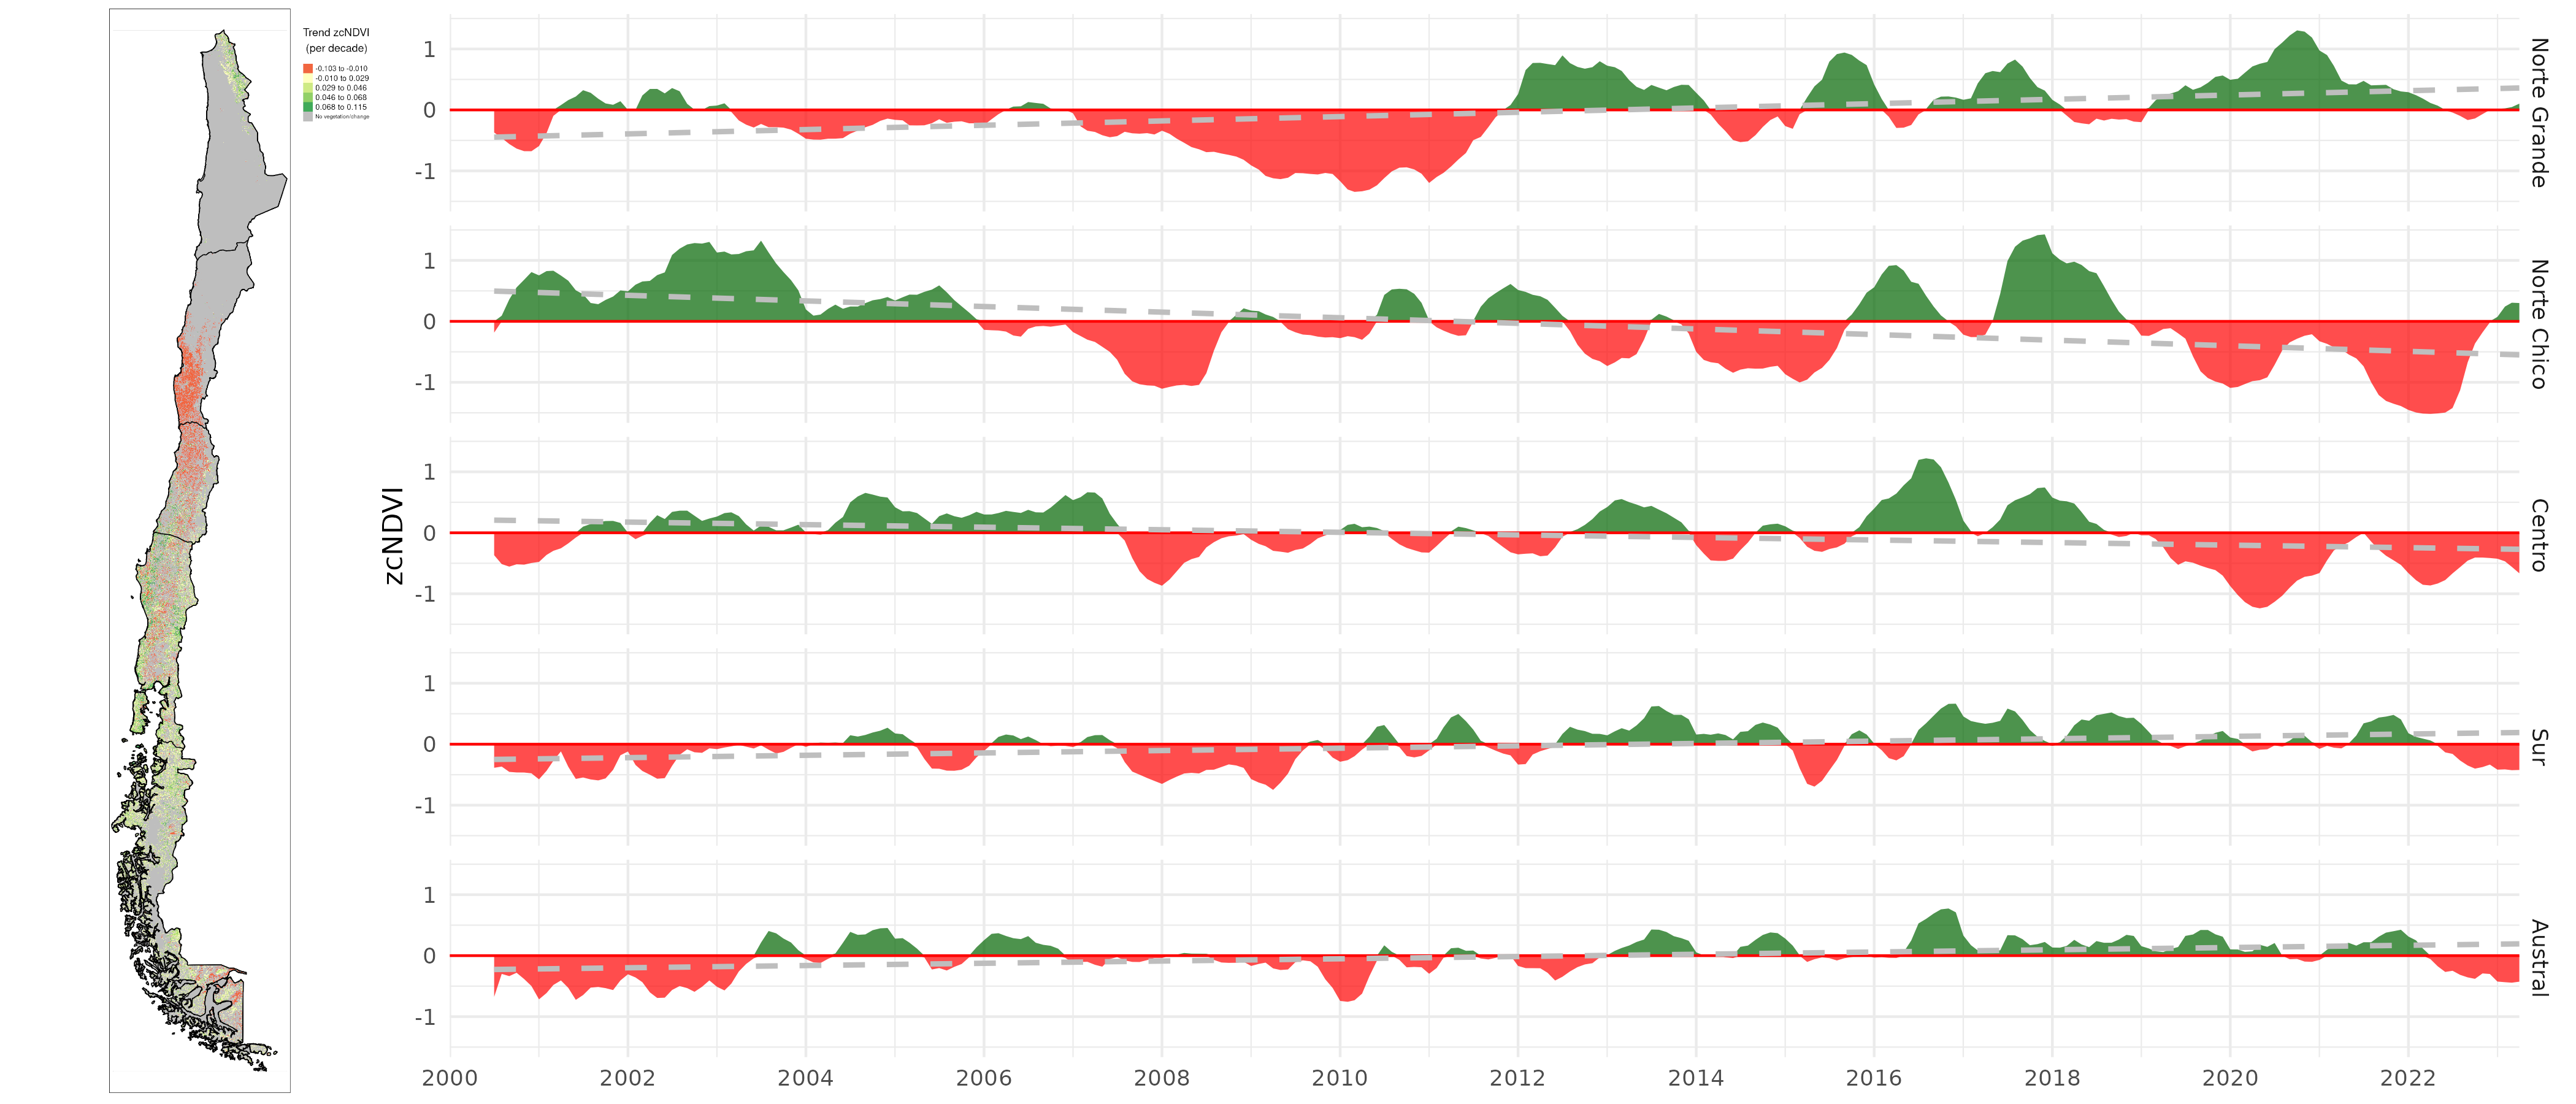
\includegraphics{../output/figs/temporal_variation_zcNDVI6_macrozonas_con_mapa.png}

}

\caption{\label{fig-zcNDVI_var}(a) Map of the linear trend of the index
zcNDVI-6 for 2001--2023. Greener colors indicate a positive trend; reder
colors correspond to a negative trend and a decrease in vegetation
productivity. Grey colors indicate either no vegetation or a change in
land cover type for 2001--2022. (b) Temporal variation of zcNDVI-6
aggregated at macrozone level within continental Chile. Each horizontal
panel corresponds to a macrozone from `Norte Grande' to `Austral'.}

\end{figure}

In Figure~\ref{fig-zcNDVI_var} it is showed the spatial map of trends in
zcNDVI (Figure~\ref{fig-zcNDVI_var}a) and the temporal variation of
zcNDVI within the aggregated macrozones (Figure~\ref{fig-zcNDVI_var}b).
In ``Norte Grande,'' vegetation productivity, as per the z-index,
exhibits a yearly increase of 0.02 with respect to grassland and
shrubland categories. There is a negative trend in ``Norte Chico'' with
-0.04 and ``Centro'' with -0.02 per decade. In the ``Norte Chico,''
savanna (-0.05) has the lowest trend, and the rest of the types are
around -0.04. In ``Centro,'' shrubland reaches -0.06, grassland -0.05,
and croplands and savanna -0.01 per decade. This could be associated
either with a reduction in vegetation surface, a decrease in biomass, or
browning \citep{Miranda2023}. Vegetation reached its lowest values since
the year 2019, with an extreme condition in early 2020 and 2022 in the
``Norte Chico'' and ``Centro''. The ``Sur'' and ``Austral'' show a
positive trend of around 0.016 per decade (Figure~\ref{fig-zcNDVI_var}).
Despite the croplands suffering from drought just as badly as the native
vegetation in ``Norte Chico,'' the savanna and shurbland appears to be
the region most affected by a negative trend in vegetation productivity.

\hypertarget{correlation-between-vegetation-productivity-and-drought-indices}{%
\subsubsection{Correlation between vegetation productivity and drought
indices}\label{correlation-between-vegetation-productivity-and-drought-indices}}

\begin{figure}[!ht]

{\centering 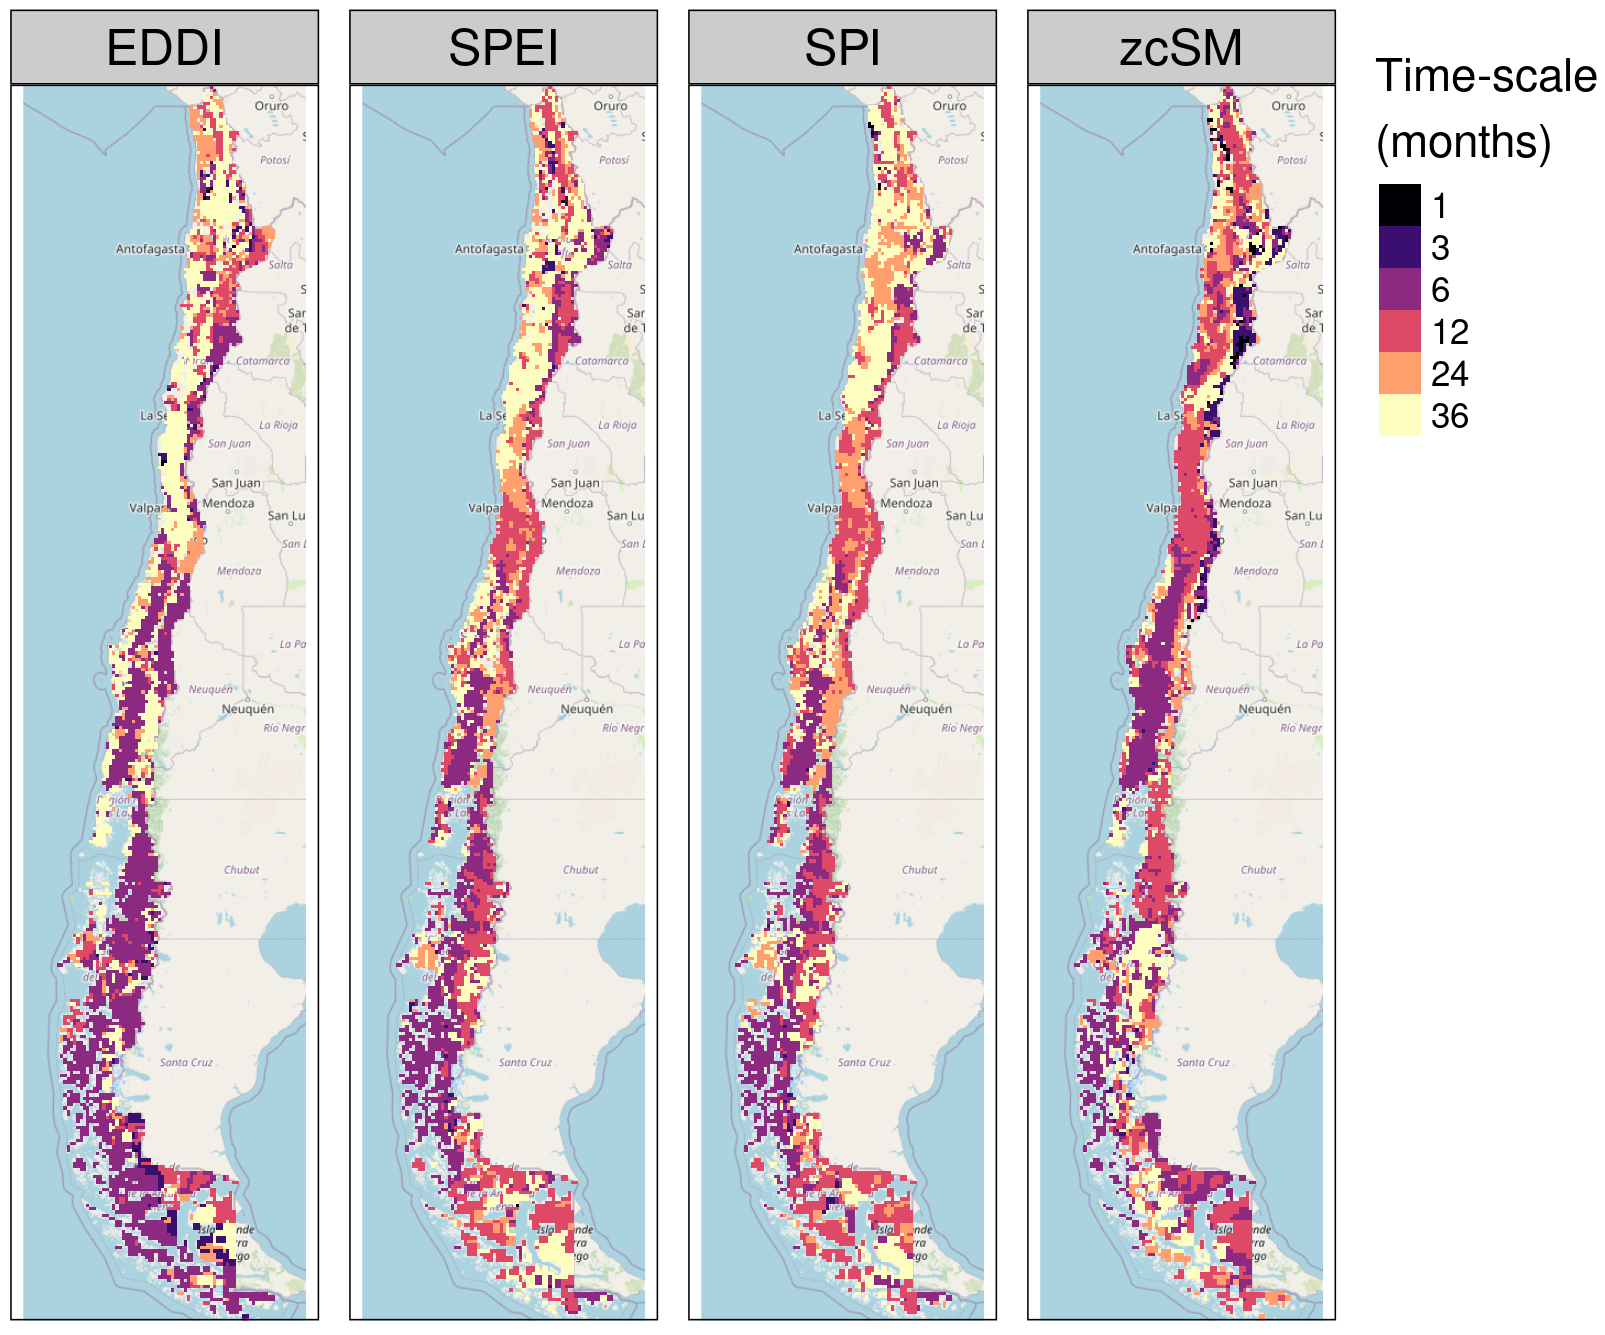
\includegraphics{../output/figs/mapa_cor_selec_indices_zcNDVI6.png}

}

\caption{\label{fig-corTimeScale}Time scales per drought index that
reach the maximum coefficient of determination}

\end{figure}

\begin{figure}[!ht]

{\centering 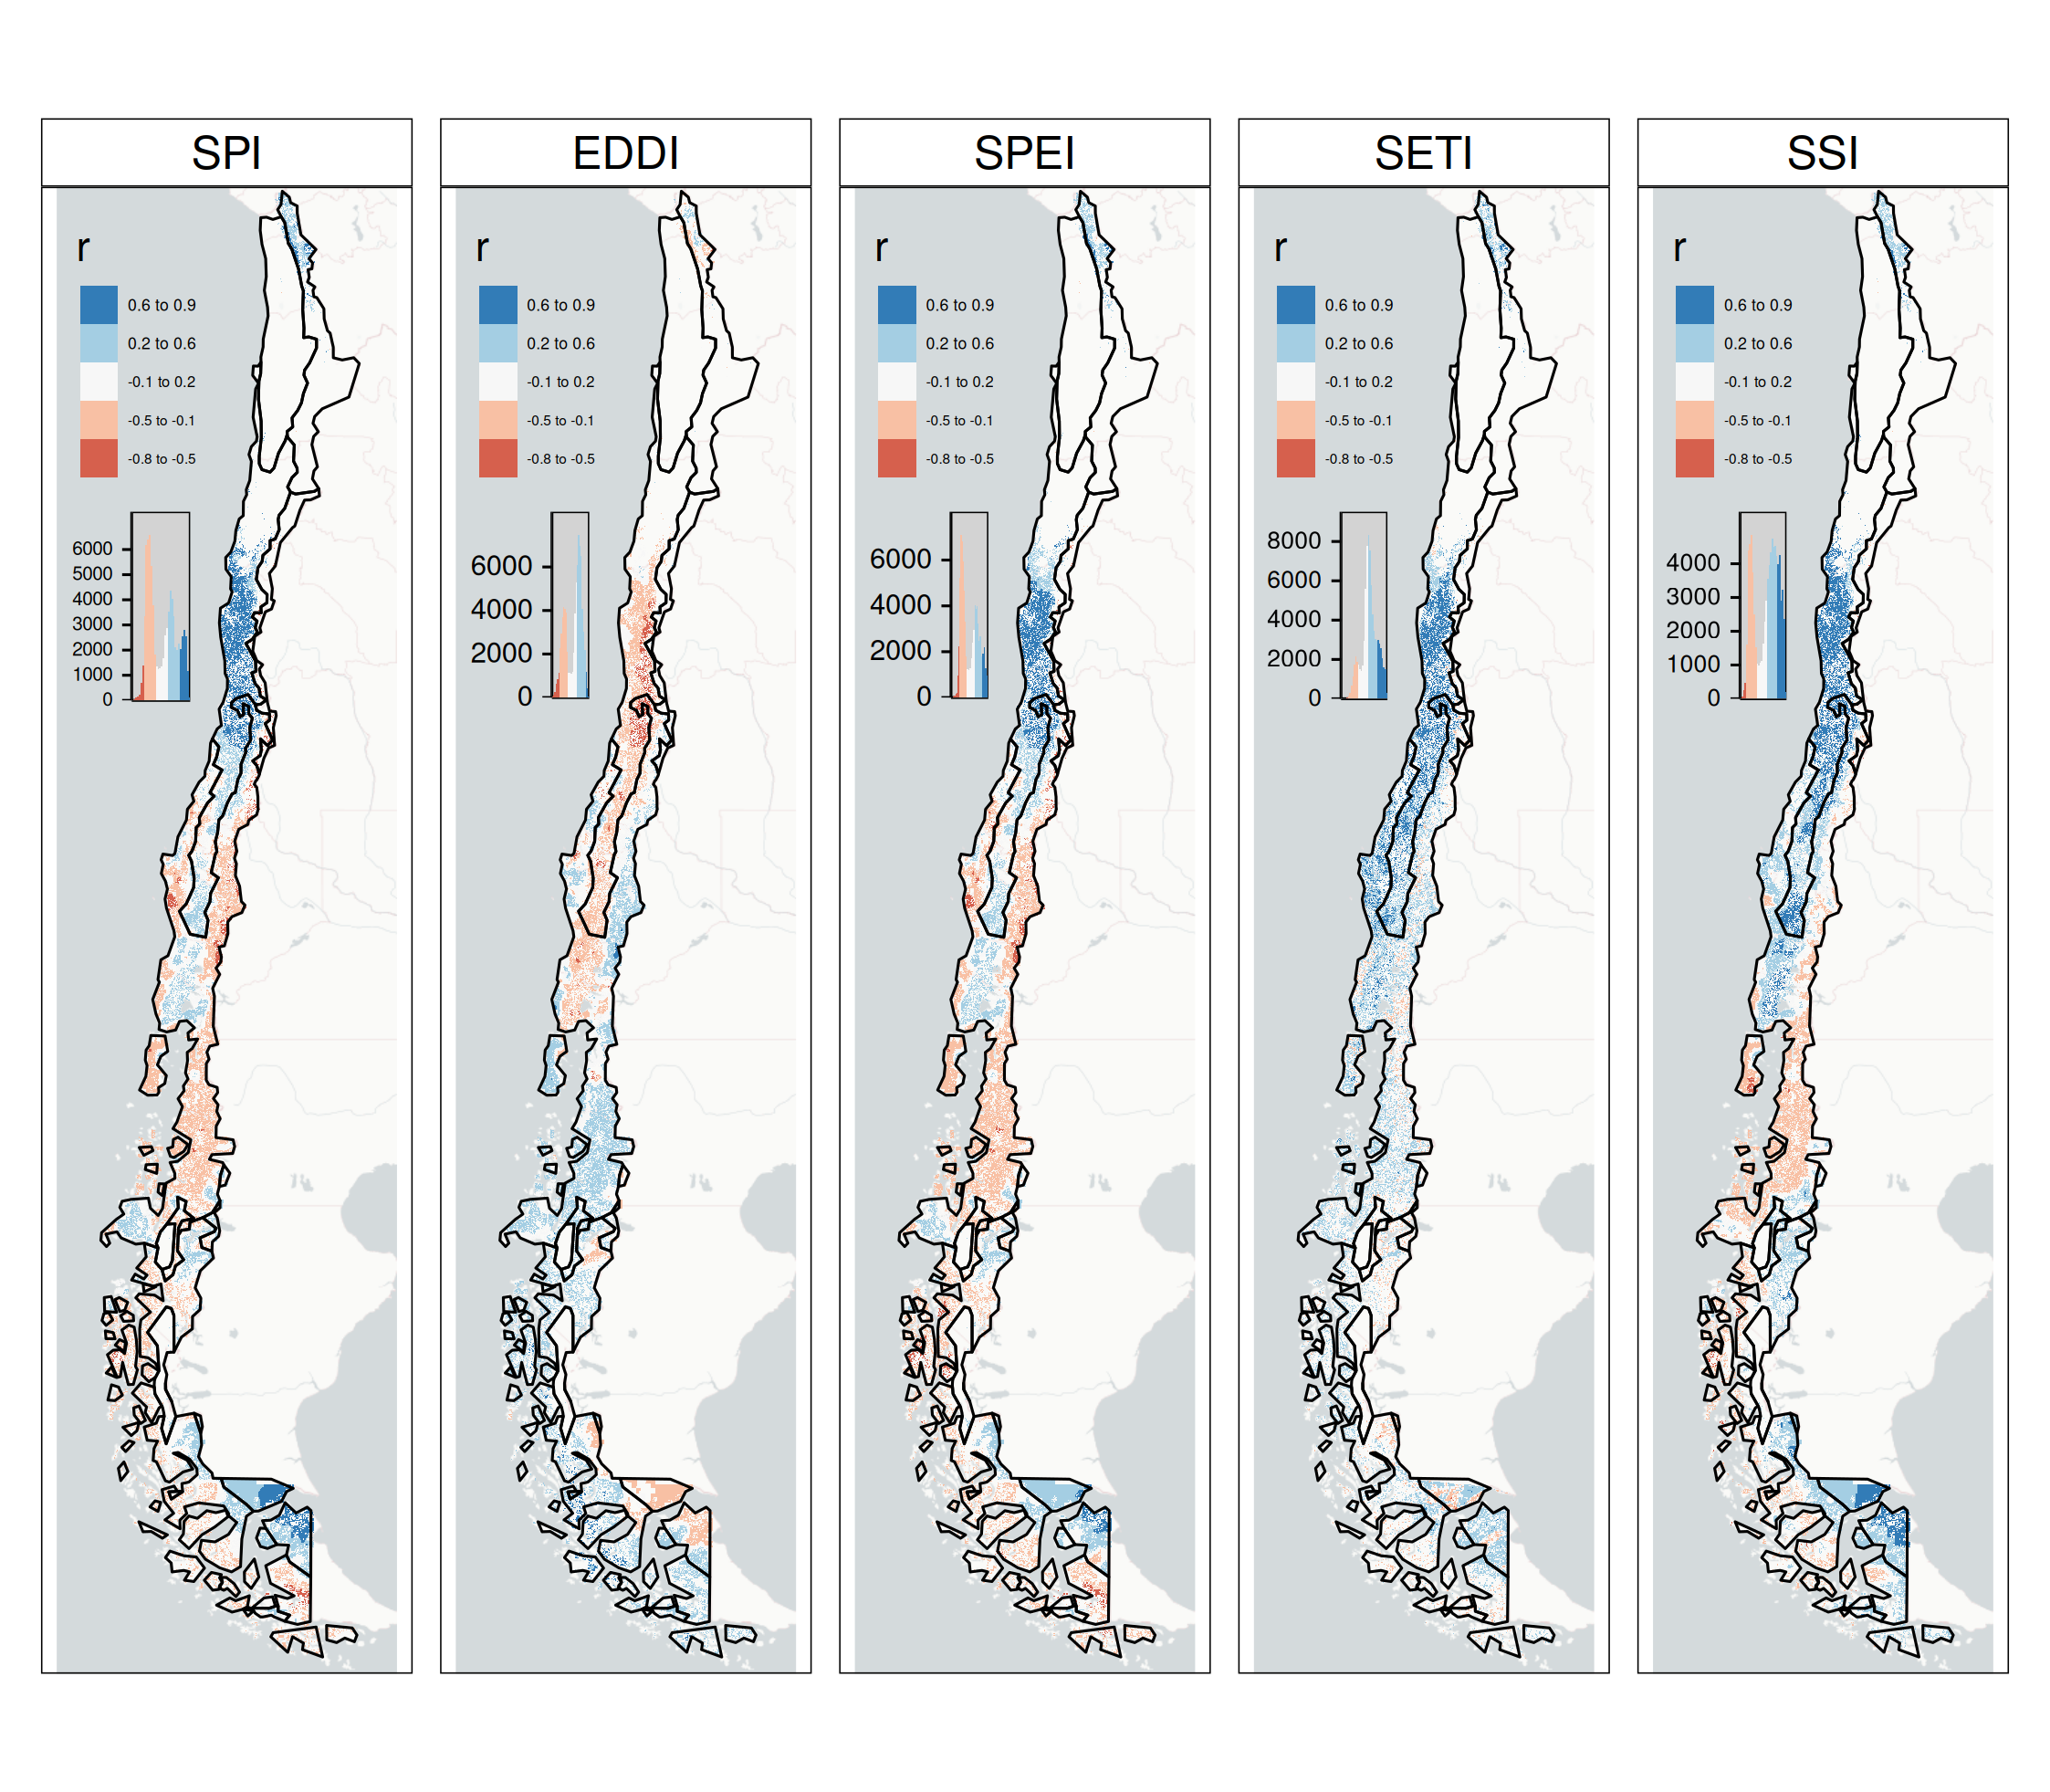
\includegraphics{../output/figs/mapa_cor_r_indices_zcNDVI6.png}

}

\caption{\label{fig-corPerson}Pearson correlation value for the time
scales and drought index that reach the maximum coefficient of
determination}

\end{figure}

Figure~\ref{fig-corTimeScale} is a map that shows the highest
coefficient of determination (r-squared, or rsq) found in the regression
analysis between different drought indicators and plant productivity
over time. The spatial variation of time scales reached per index is
mostly for time scales above 12 months. In the case of SSI, the
predominant scales are 6 and 12 months. For all indices, to the north,
the time scales are higher and diminish toward the south until the south
part of ``Austral'' increases. In Figure~\ref{fig-corPerson}, the map of
Pearson correlation values is shown. The EDDI reached correlations above
0.5 between ``Norte Chico'' and ``Sur.'' The correlation changes from
negative to positive toward the Andes Mountains and to the sea, just as
in the northern part of ``Austral.'' The SPI and SPEI have similar
results, with the higher values in ``Norte Chico'' and ``Centro'' being
higher than 0.6. Following a similar spatial pattern as EDDI. The SSI
showed to be the index that has a major spatial extension with a higher
correlation. It has a similar correlation to SPI and SPEI for ``Norte
Chico'' and ``Sur,''~ but has improvements for ``Sur.''

\begin{table}[!ht]
\caption{Summarry per land cover macroclass and macrozone regarding the correlation between zcNDVI with the drought indices EDDI, SPI, SPEI, and SSI for time scales of 1, 3, 6, 12, 24, and 36. The numbers in each cell indicate the time scale that reached the maximum correlation for the land cover and macrozone, and the color indicates the strength of the r-squared obtained with the index and the time scale.}
\label{tab-corlandcover}
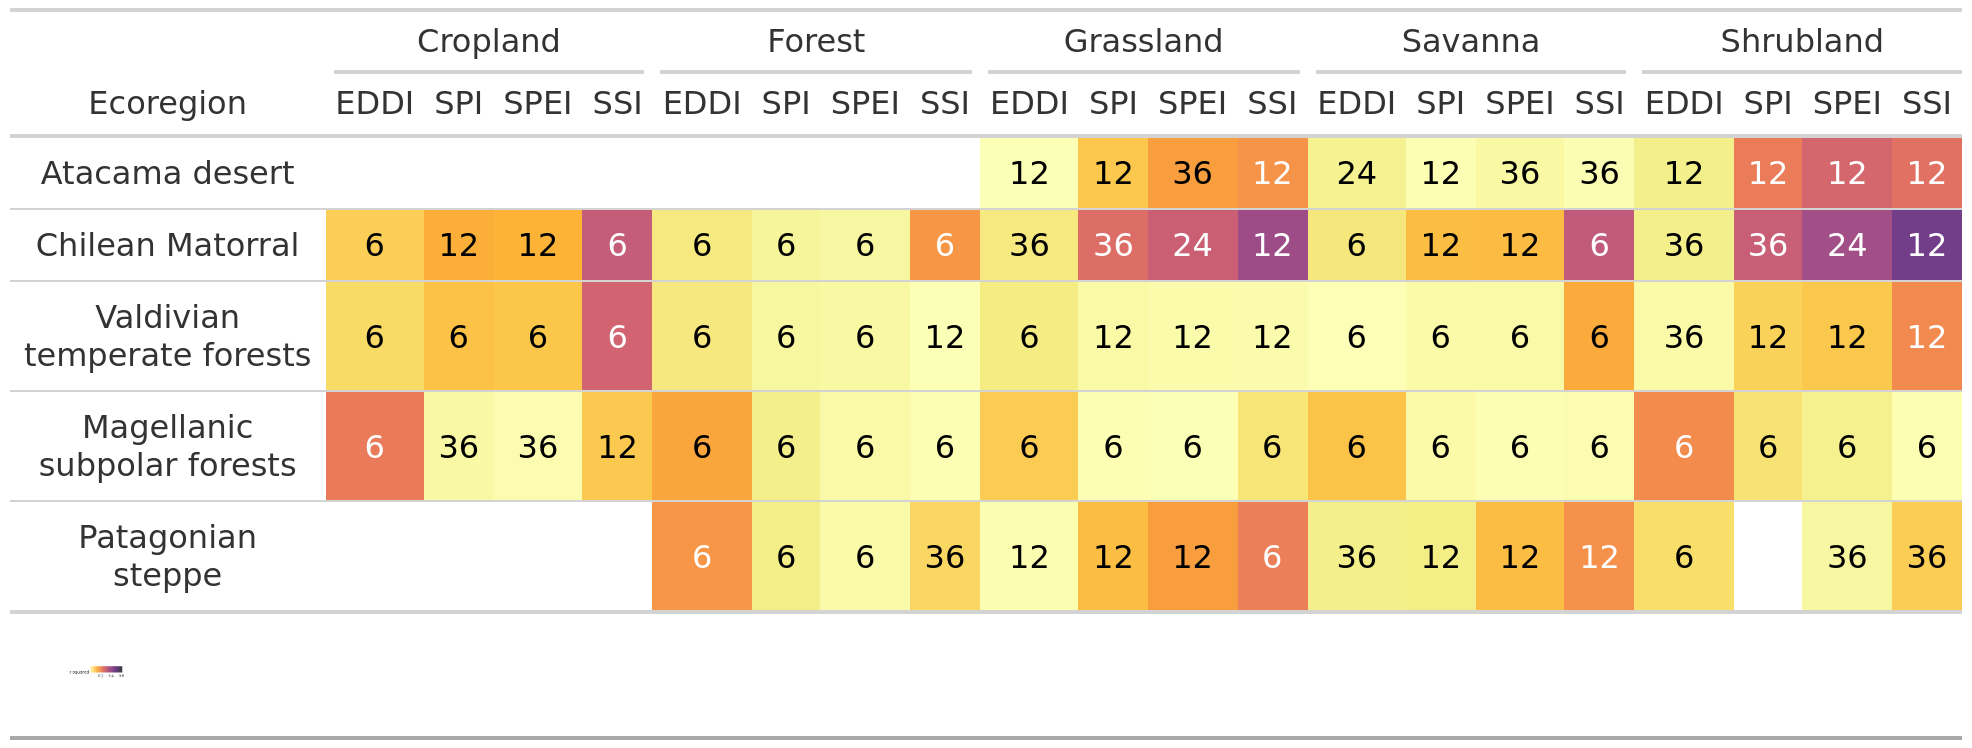
\includegraphics[]{../output/figs/tabla_r_cor_macro_indice.png}
\end{table}

In Table \ref{tab-corlandcover}, we aggregate per macrozone and
landcover the correlation analysis presented in
Figure~\ref{fig-corTimeScale} and Figure~\ref{fig-corPerson}. According
to what is shown, forests seem to be the most resistant to drought.
Showing that only ``Centro'' is slightly (rsq = 0.25) impacted by a
12-month soil moisture deficit (SSI-12). In the ``Norte Chico'' and to a
lesser extent in the ``Norte Grande,'' it is evident that a SSI-12 with
a rsq = 0.45 and a decrease in water supply (SPI-36 and SPEI-24 with rsq
= 0.28 and 0.34, respectively) have an impact on grasslands. However,
this type was unaffected by soil moisture, water supply, or demand in
macrozones further south. The types that show to be most affected by
variation in climate conditions are shrublands, savannas, and croplands.
For savannas in ``Norte Chico,'' the SSI-12 and SPI-24 reached an rsq of
0.74 and 0.58, respectively. This value decreases to the south, but the
SSI-12 is still the variable explaining more of the variation in
vegetation productivity (rsq = 0.45 in ``Centro'' and 0.2 in ``Sur'').
In the case of croplands, the SPEI-12, SPI-36, and SSI-12 explain
between 45\% and 66\% of the variability in ``Norte Chico.'' The type of
land most impacted by climatic variation was shrubland, where soil
moisture explained 59\% and precipitation, 37\%, in ``Norte Chico'' and
``Centro,'' with SSI-12 being the most relevant variable, then SPI-36 in
``Norte Chico'' and SPI-24 in ``Sur.''

\hypertarget{discussion}{%
\section{Discussion}\label{discussion}}

\hypertarget{drought-trend-and-attribution-to-land-cover}{%
\subsection{Drought trend and attribution to land
cover}\label{drought-trend-and-attribution-to-land-cover}}

\citet{Vicente-Serrano2022}, in a study at the global scale of drought
trends, indicate that there have not been significant trends in
meteorological drought since 1950. Also, state that the increase in
hidrological trend in some parts of the globe (northeast Brazil and the
Mediterranean region) is related to changes in land cover and
specifically to the rapidly increasing irrigated area, which
consequently increases water extraction. \citet{Kogan2020} analyzed the
agricultural drought impact globally and in the main grain producer
countries, finding that \emph{``since 1980, the Earth warming has not
changed the drought area or intensity.''} In our study, we considered
the variation in vegetation productivity in Chile for areas without
changes in land cover, to avoid misleading conclusions that could be
related to the increase in water demand due to land cover change. Our
results show a contrasting perspective. There has been a significant
trend in the decline of vegetation productivity (zcNDVI) since 2000 for
``Norte Chico'' and ``Centro,'' which has been extreme between 2020 and
2022, seemsly due to an intense hydrological drought due to the
persistance of the mega drought \citep{Garreaud2017}. However, a rise in
irrigated land doesn't seem to have an impact on this hydrological
drought. Despite using the persistance mask for vegetation's trend
analysis, cropland, which is the most water-demand type, showed a
decrease trend in ``Norte Chico'' and ``Centro.'' Also, there was an
increase in barren land for both types. These changes are associated
with a decrease in water demand from vegetation. Nonetheless, we used
the persistant land cover to ensure that the pixel has the same class;
in the case of croplands, it could happen that some areas had changed
crops for others with higher water consumption and consequently increase
water demand. But this effect should be minor compared to the results
from land cover change at this scale of analysis.

On the other hand, for ``Norte Chico'' and ``Centro,'' our results show
a decrease in trends of water supply (SPI and SSI), which are higher at
larger time scales, which is evidence of the hydrological drought. We
say that what happened in central Chile goes against what has been found
on a global scale \citep{Vicente-Serrano2022, Kogan2020}. This shows
that the main cause of the hydrological drought in Chile was a steady
drop in water supply made worse by an increase in AED, but it seems that
in zones most affected by drought, the main cause is not an increase in
water demand by vegetation like irrigated crops. Finally, north-central
Chile has experienced a decline in vegetation productivity across all
macroclasses, which is primarily attributable to variations in water
supply and soil moisture. An increase in water demand, such as an
increase in the surface area of irrigated crops, could strengthen this
trend.

\hypertarget{land-cover-types-and-their-impact-by-drought}{%
\subsection{Land cover types and their impact by
drought}\label{land-cover-types-and-their-impact-by-drought}}

We discovered that croplands, savannas, and shrubland are the most
susceptible to climatic changes and are most affected by the 12-month
soil moisture deficit. In a study in the Yangtze River Basin in China,
\citet{Jiang2020} analyzed the impact of drought on vegetation using the
SPEI and the Enahanced Vegetation Index (EVI). They found that cropland
was more sensitive to drought than grassland, showing that cropland
responds strongly to short- and medium-term drought (\textless{}
SPEI-6). In our case, the SPEI-12 was the one that most impacted the
croplands in ``Norte Chico'' and ``Centro.'' In general, most studies
show that croplands are most sensitive to short-term drought
(\textless{} SPI-6)
\citep{Zambrano2016, Potopova2015, Dai2020, Rhee2010}. Short-term
precipitation deficits impact soil water, and thus less water is
available for plant growth. However, we found that in ``Norte Chico,''
an SPI-36 and SPEI-12 had a higher impact, which are associated with
hydrological drought (long-term), and in ``Centro,'' an SPI-12 and
SPEI-12. Thus, we attribute this impact to the hydrological drought that
has decreased groundwater storage \citep{Taucare2024}, which in turn is
impacted by long-term deficits, and consequently, the vegetation is more
dependent on groundwater. In ``Sur'' and ``Austral,'' the correlations
between drought indices and vegetation productivity decrease, as do the
time scales that reach the maximum r-squared. What can be explained is
that, south of ``Centro,'' predominate forest and grassland, the most
resistant types. Also, drought episodes have been less frequent and
intense. The drought episodes have had a lower impact on water
availability for vegetation.

According to \citet{Senf2020}, severe drought conditions in Europe are a
significant cause of tree mortality. However, we found that forest is
the type of land cover macroclass less affected by variation in drought
indices, being the most resistant land cover class to drought.
Supporting this is \citet{Fathi-Taperasht2022}{]}, who assert that
Indian forests are the most drought-resistant and recover rapidly.
Similarly, the work of \citet{Wu2024}, who analyzed vegetation loss and
recovery in response to meteorological drought in the humid subtropical
Pearl River basin in China, indicates that forests showed higher drought
resistance. Using Vegetation Optical Depth (VOD), kNDVI, and EVI,
\citet{Xiao2023} test the resistance of ecosystems and find that
ecosystems with more forests are better able to handle severe droughts
than croplands. They attribute the difference to a deeper rooting depth
of trees, a higher water storage capacity, and different water use
strategies between forest and cropland \citep{Xiao2023}.

In contrast to what we obtained, \citet{Venegas2022}, who studied
Cryptocarya alba and Beilschmiedia miersii (both from the Lauraceae
family) that live in sclerophyllous forests in Chile, found that the
trees' overall growth had slowed down. This could mean that the natural
dynamics of their forests have changed. They attributed it to the
cumulative effects of the unprecedented drought (i.e., hydrological
drought). Thus, we attribute that forest to being the most resistant to
drought, due to the fact that most of the species comprising it are
highly resilient to water scarcity compared to the other land cover
classes. Nonetheless, if we want to go deep in our analysis, we should
use earth observation data that is able to capture a higher level of
detail. For example, when we used MOD13A3 with a 1km spatial resolution
to measure vegetation condition, it took the average condition of 1
square kilometer. Then, to use remote sensing to look at how a certain
type of forest (like sclerophyllous forest) changes in response to
drought on a local level, we should use operational products with higher
spatial resolutions, like those from Landsat or Sentinel. This will let
us do a more thorough analysis.

\hypertarget{soil-moisture-vegetation-productivity-and-agricultural-drought.}{%
\subsection{Soil moisture, vegetation productivity, and agricultural
drought.}\label{soil-moisture-vegetation-productivity-and-agricultural-drought.}}

The main external factors that affect biomass production by vegetation
are actual evapotranspiration and soil moisture, and the rate of ET in
turn depends on the availability of water storage in the root zone.
Thus, soil moisture plays a key role in land carbon uptake and,
consequently, in the production of biomass \citep{Humphrey2021}.
Moreover, \citet{Zhang2022} indicate there is a bidirectional causality
between soil moisture and vegetation productivity. Lastly, some studies
have redefined agricultural drought as soil moisture drought from a
hydrological perspective \citep{Loon2016, Samaniego2018}. Even though
soil moisture is the external factor most determinant of vegetation
biomass, there are multiple internal factors, such as species,
physiological characteristics, and plant hydraulics, that would affect
vegetation productivity. Because of that, we believe that agricultural
drought, referring to the drought that impacts vegetation productivity,
is the most proper term, as originally defined by \citet{Wilhite1985}.

The study results showed that the soil moisture-based drought index
(SSI) was better at explaining vegetation productivity across land cover
macroclasses than meteorological drought indices like SPI, SPEI, and
EDDI. In the early growing season and especially in irrigated rather
than rainfed croplands, soil moisture has better skills than SPI and
SPEI for estimating gross primary production (GPP). This according to
\citet{Chatterjee2022} evaluation of the SPI and SPEI and their
correlation with GPP in the CONUS. Also, \citet{Zhou2021} indicate that
the monthly scaled Standardized Water Deficit Index (SWDI) can
accurately show the effects of agricultural drought in most of China.
\citet{Nicolai2017} also looked at the time-lag between the SWDI and the
Vegetation Condition Index (VCI). They found that there was little to no
time-lag in croplands but a greater time-lag in forests.

In our case, there is strong spatial variability throughout Chile and
between classes, mainly attributable to climate heterogeneity,
hydrological status, or vegetation resistance to water scarcity. The
semi-arid ``Norte Chico'' and the Mediterranean ``Centro'' were where
SSI had the best performance. In Chile, medium-term deficits of 12
months are more relevant in the response of vegetation, which decreases
to the south, and in the case of croplands, they seem to react in a
shorter time, with six months (SSI-6) in ``Centro.'' This variation for
croplands could be related to the fact that in ``Norte Chico,'' the
majority of crops are irrigated, but to the south there is a higher
proportion of rainfed agriculture, which is most dependent on the
short-term availability of water. Rather, in the ``Norte Chico,'' the
orchards are more dependent on the storage of water in dams of
groundwater reservoirs, which are affected by long-term drought (e.g.,
SPI-36).

\hypertarget{future-outlook-to-complete}{%
\subsection{Future outlook (to
complete)}\label{future-outlook-to-complete}}

\hypertarget{conclusion}{%
\section{Conclusion}\label{conclusion}}

There is a trend toward decreasing water supply in most parts of Chile,
particularly in the ``Centro'' and ``Norte Chico'' regions. The whole
country showed an increase in AED. Vegetation productivity only showed a
decrease in the ``Norte Chico'' and ``Centro,'' being highest for
shrubland and croplands. Forest is the land cover most resistant to
drought, as shown along Chile, and shrubland and cropland are the most
sensitive.

A soil moisture deficit of 12 months (SSI-12) is highly correlated with
vegetation productivity for the land cover classes of shrubland,
savannas, croplands, and forest in ``Norte Chico'' and ``Centro.'' For
the southern part of the country with humid conditions, the correlation
with SSI decreases. Soil moisture overcomes the capacity to explain
vegetation productivity over the supply and demand drought indices in
the entire territory.

The variation in vegetation productivity appears to be associated with
climate variation rather than anthropogenic factors (e.g., an increase
in water demand by irrigated crops). Even though switching to more
demanding crops on the land could increase the impact of drought on
vegetation, this would need to be more thoroughly investigated, for
instance at the watershed level.

The results of this study could help in the development of a robust
forecasting system for land cover classes in Chile, helping to improve
preparedness for climate change impacts on vegetation.

\hypertarget{supplementary-material}{%
\section*{Supplementary material}\label{supplementary-material}}
\addcontentsline{toc}{section}{Supplementary material}


\renewcommand\refname{References}
  \bibliography{references.bib}


\end{document}
